%definira klasu dokumenta
\documentclass[12pt]{report}

%prostor izmedu naredbi \documentclass i \begin{document} se zove uvod. U njemu se nalaze naredbe koje se odnose na cijeli dokument

%osnovni LaTex ne može riješiti sve probleme, pa se koriste različiti paketi koji olakšavaju izradu željenog dokumenta
\usepackage[croatian]{babel}
\usepackage{amssymb}
\usepackage{amsmath}
\usepackage{txfonts}
\usepackage{mathdots}
\usepackage{titlesec}
\usepackage{array}
\usepackage{lastpage}
\usepackage{etoolbox}
\usepackage{tabularray}
\usepackage{color, colortbl}
\usepackage{adjustbox}
\usepackage{geometry}
\usepackage[classicReIm]{kpfonts}
\usepackage{hyperref}
\usepackage{fancyhdr}
\usepackage{listings}
\usepackage{float}
\usepackage{setspace}
\restylefloat{table}


\patchcmd{\chapter}{\thispagestyle{plain}}{\thispagestyle{fancy}}{}{} %redefiniranje stila stranice u paketu fancyhdr

%oblik naslova poglavlja
\titleformat{\chapter}{\normalfont\huge\bfseries}{\thechapter.}{20pt}{\Huge}
\titlespacing{\chapter}{0pt}{0pt}{40pt}


\linespread{1.3} %razmak između redaka

\geometry{a4paper, left=1in, top=1in,}  %oblik stranice

\hypersetup{ colorlinks, citecolor=black, filecolor=black, linkcolor=black,	urlcolor=black }   %izgled poveznice


%prored smanjen između redaka u nabrajanjima i popisima
\newenvironment{packed_enum}{
	\begin{enumerate}
		\setlength{\itemsep}{0pt}
		\setlength{\parskip}{0pt}
		\setlength{\parsep}{0pt}
	}{\end{enumerate}}

\newenvironment{packed_item}{
	\begin{itemize}
		\setlength{\itemsep}{0pt}
		\setlength{\parskip}{0pt}
		\setlength{\parsep}{0pt}
	}{\end{itemize}}




%boja za privatni i udaljeni kljuc u tablicama
\definecolor{LightBlue}{rgb}{0.9,0.9,1}
\definecolor{LightGreen}{rgb}{0.9,1,0.9}

%Promjena teksta za dugačke tablice
\DefTblrTemplate{contfoot-text}{normal}{Nastavljeno na idućoj stranici}
\SetTblrTemplate{contfoot-text}{normal}
\DefTblrTemplate{conthead-text}{normal}{(Nastavljeno)}
\SetTblrTemplate{conthead-text}{normal}
\DefTblrTemplate{middlehead,lasthead}{normal}{Nastavljeno od prethodne stranice}
\SetTblrTemplate{middlehead,lasthead}{normal}

%podesavanje zaglavlja i podnožja

\pagestyle{fancy}
\lhead{Programsko inženjerstvo}
\rhead{$<$SkillEtCooking$>$}
\lfoot{$<$Progimeri$>$}
\cfoot{stranica \thepage/\pageref{LastPage}}
\rfoot{\today}
\renewcommand{\headrulewidth}{0.2pt}
\renewcommand{\footrulewidth}{0.2pt}


\begin{document}



\begin{titlepage}
	\begin{center}
		\vspace*{\stretch{1.0}} %u kombinaciji s ostalim \vspace naredbama definira razmak između redaka teksta
		\LARGE Programsko inženjerstvo\\
		\large Ak. god. 2021./2022.\\

		\vspace*{\stretch{3.0}}

		\huge SkillEtCooking\\
		\Large Dokumentacija, Rev. 2.\\

		\vspace*{\stretch{12.0}}
		\normalsize
		Grupa: \textit{$Progimeri$}\\
		Voditelj: \textit{Karlo Frankola}\\


		\vspace*{\stretch{1.0}}
		Datum predaje: \textit{14. siječnja 2022.}\\

		\vspace*{\stretch{4.0}}

		Nastavnik: \textit{Eugen Vušak, mag. ing. comp}\\

	\end{center}


\end{titlepage}


\tableofcontents


\chapter{Dnevnik promjena dokumentacije}




\begin{longtblr}[
	label=none
	]{
		width = \textwidth,
		colspec={|X[2]|X[13]|X[4]|X[4]|},
		rowhead = 1
	}
	\hline
	\textbf{Rev.}	& \textbf{Opis promjene/dodatka} & \textbf{Autori} & \textbf{Datum}\\[3pt] \hline
	0.1 & Napravljen predložak & Karlo Frankola & 15.10.2021. 		\\[3pt] \hline
	0.2	& Opis projektnog zadatka & Dario Dugonjevac & 28.10.2021. 	\\[3pt] \hline
	0.3 & Dodani funkcionalni zahtjevi & Borna Colarić & 31.10.2021. \\[3pt] \hline
	0.4 & Dodani obrasci uporabe & Toni Serezlija & 01.11.2021. \\[3pt] \hline
	0.5 & Napravljeni dijagrami obrazaca uporabe & Marko Tunjić & 02.11.2021. \\[3pt] \hline
	0.6 & Sekvencijski dijagrami & Dario Dugonjevac & 12.11.2021. \\[3pt] \hline
	0.7 & Definirani nefunkcionalni zahtjevi & Toni Serezlija & 13.11.2021. \\[3pt] \hline
	0.8 & Opis tablica baze podataka & Karlo Frankola & 14.11.2021. \\[3pt] \hline
	0.9 & Dijagram baze podataka & Marko Tunjić & 15.11.2021. \\[3pt] \hline
	0.10 & Dijagram razreda & Jan Brkić & 16.11.2021. \\[3pt] \hline
	0.10.1 & Dopunjeni dijagrami razreda & Karlo Frankola & 19.11.2021. \\[3pt] \hline
	\textbf{1.0} & Dopuna dnevnika aktivnosti i prva predaja & Karlo Frankola & 19.11.2021. \\[3pt] \hline
	1.1 & Dodana dokumentacija za ispitivanje komponenti & Marko Tunjić & 13.01.2021. \\[3pt] \hline
	1.2 & Dodani dijagrami stanja i aktivnosti & Jan Brkić & 13.01.2021. \\[3pt] \hline
	1.3 & Dodan dijagram razreda i razmještaja, upute za pokretanje & Karlo Frankola & 14.01.2021. \\[3pt] \hline
	1.4 & Dodan zaključak, dijagram komponenti, korištene tehnologije & Dario Dugonjevac & 14.01.2021. \\[3pt] \hline
	1.5 & Popravak dijagrama stanja & Jan Brkić & 14.01.2021. \\[3pt] \hline
	1.6 & Dopuna prikaza aktivnosti grupe & Karlo Frankola & 14.01.2021. \\[3pt] \hline
	\textbf{2.0} & Predaja druge revizije & Karlo Frankola & 14.01.2021. \\[3pt] \hline

\end{longtblr}

\chapter{Opis projektnog zadatka}

Cilj ovog projekta je razviti programsku potporu za stvaranje web aplikacije \textit{"SkillEtCooking"} koja će korisniku olakšati snalaženje u kuhinji i optimizaciju iskorištavanja sastojaka koje osoba već posjeduje. Na taj način korisnik neće morati provesti cijeli dan razmišljajući što i kako napraviti nego to aplikacija radi umjesto njega.
\newline Sustav će podržavati više vrsta korisnika:
\begin{packed_item}
	\item registrirani
	\item neregistrirani
	\item moderatori.
\end{packed_item}

Neregistriranim korisnicima se prilikom otvaranja aplikacije otvori početna stranica na kojoj se nalaze svi recepti (\ref{fig:promjene}). Recepti se mogu sortirati na razne načine:

\begin{packed_item}
	\item popularnost
	\item prosječna ocjena recepta
	\item oznaka "Preporučeno".
\end{packed_item}

Popularnost se određuje na osnovu broja otvaranja pojedinog recepta dok se sortiranje po oznaci "Preporučeno" određuje na osnovu prosjeka popularnosti i prosječne ocjene koristeći funkciju:

\begin{packed_item}
	\item ocjena/prosjecnaOcjena + brojOtvaranja/prosjecniBrojOtvaranja
\end{packed_item}

\begin{figure}[H]
	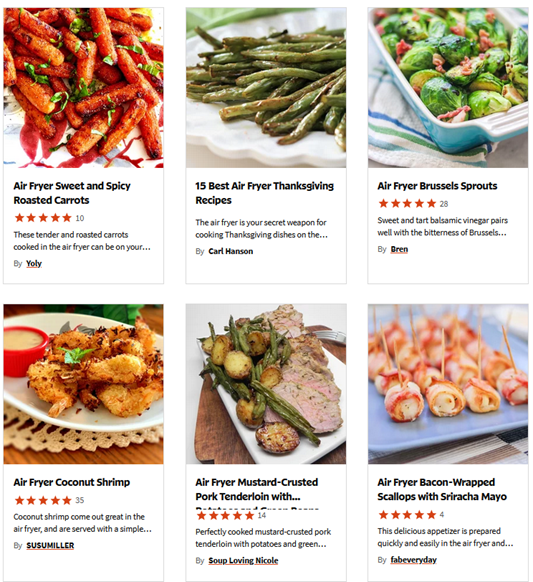
\includegraphics[scale=0.8]{slike/Slika1.PNG} %veličina slike u odnosu na originalnu datoteku i pozicija slike
	\centering
	\caption{Prikaz svih recepata}
	\label{fig:promjene}
\end{figure}
Neregistrirani korisnici imaju mogućnost filtriranja recepata upisivanjem imena recepta ili sastojka/sastojaka. Nakon filtriranja skupa recepata po sastojcima, recepti se sortiraju po vrijednosti Jaccardovog indeksa sličnosti s time da najsličniji dolazi prvi te se izbacuju svi recepti čija je vrijednost indeksa sličnosti manja od praga. Za to vrijeme, ostali izbori sortiranja su onemogućeni, ali pretraživanje po naslovu je i dalje u funkciji.

Sljedeća mogućnost neregistriranih korisnika je da im se pritiskom na naziv recepta prikazuje stranica s detaljima recepta. Na toj stranici vidljivi su svi podatci vezani za recept:

\begin{packed_item}
	\item slika
	\item naziv
	\item procijenjeno vrijeme kuhanja
	\item sastojci i količina svakog sastojka
	\item koraci pripreme s kratkim opisom
	\item ocjena (\ref{fig:promjene2}).
\end{packed_item}

\begin{figure}[H]
	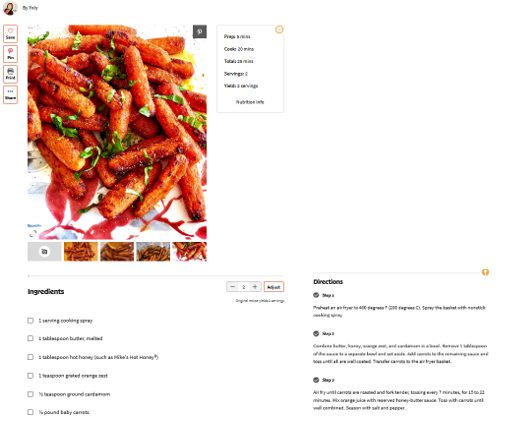
\includegraphics[scale=0.8]{slike/Slika2.PNG} %veličina slike u odnosu na originalnu datoteku i pozicija slike
	\centering
	\caption{Primjer otvorenog recepta}
	\label{fig:promjene2}
\end{figure}

Stranica sadrži prostor sa komentarima i ocjenama gdje je moguće vidjeti iskustva drugih korisnika što će biti izvedeno korištenjem Disqus usluge (\ref{fig:promjene3}). Tu je vidljiva prva razlika između registriranog i neregistriranog korisnika, a to je da komentare i ocjene mogu ostaviti samo registrirani korisnici. Također ukoliko je autor ostavio komentar na svoj recept, komentar će biti dodatno naglašen i bolje uočljiv ostalim korisnicima.

Osim toga, stranica sadrži i mogućnost da klikom na gumb korisnik može pregledati sve ostale recepte s istim autorom kao i odabrani recept.

Registrirani korisnik se može prijaviti, a neregistrirani će imati mogućnost registracije u sustav (\ref{fig:promjene4}). Prijavljeni korisnik može koristiti aplikaciju na jednak način kao i neprijavljeni korisnik, ali prijavljeni korisnik također može dodavati i uređivati vlastite recepate, uređivati vlastite podatke te koristiti prethodno objašnjenu funkcionalnost ostavljanja komentara. Pravila prilikom unosa recepta su da korisnik mora unijeti sliku jela (maksimalno 5), barem jedan sastojak i količinu te barem jedan korak pripreme.
\begin{figure}[H]
	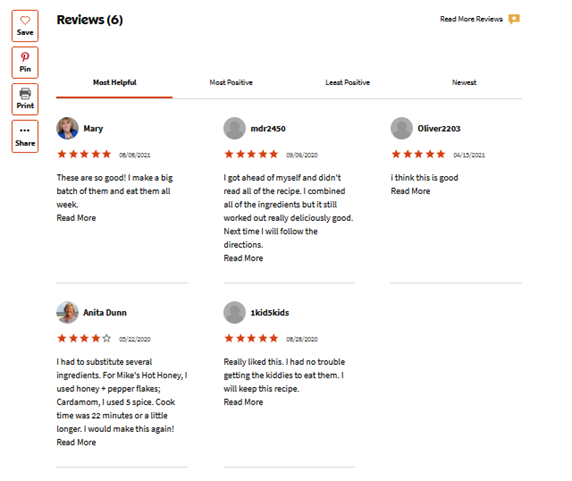
\includegraphics[scale=0.8]{slike/Slika3.PNG} %veličina slike u odnosu na originalnu datoteku i pozicija slike
	\centering
	\caption{Komentari na recept}
	\label{fig:promjene3}
\end{figure}

\begin{figure}[H]
	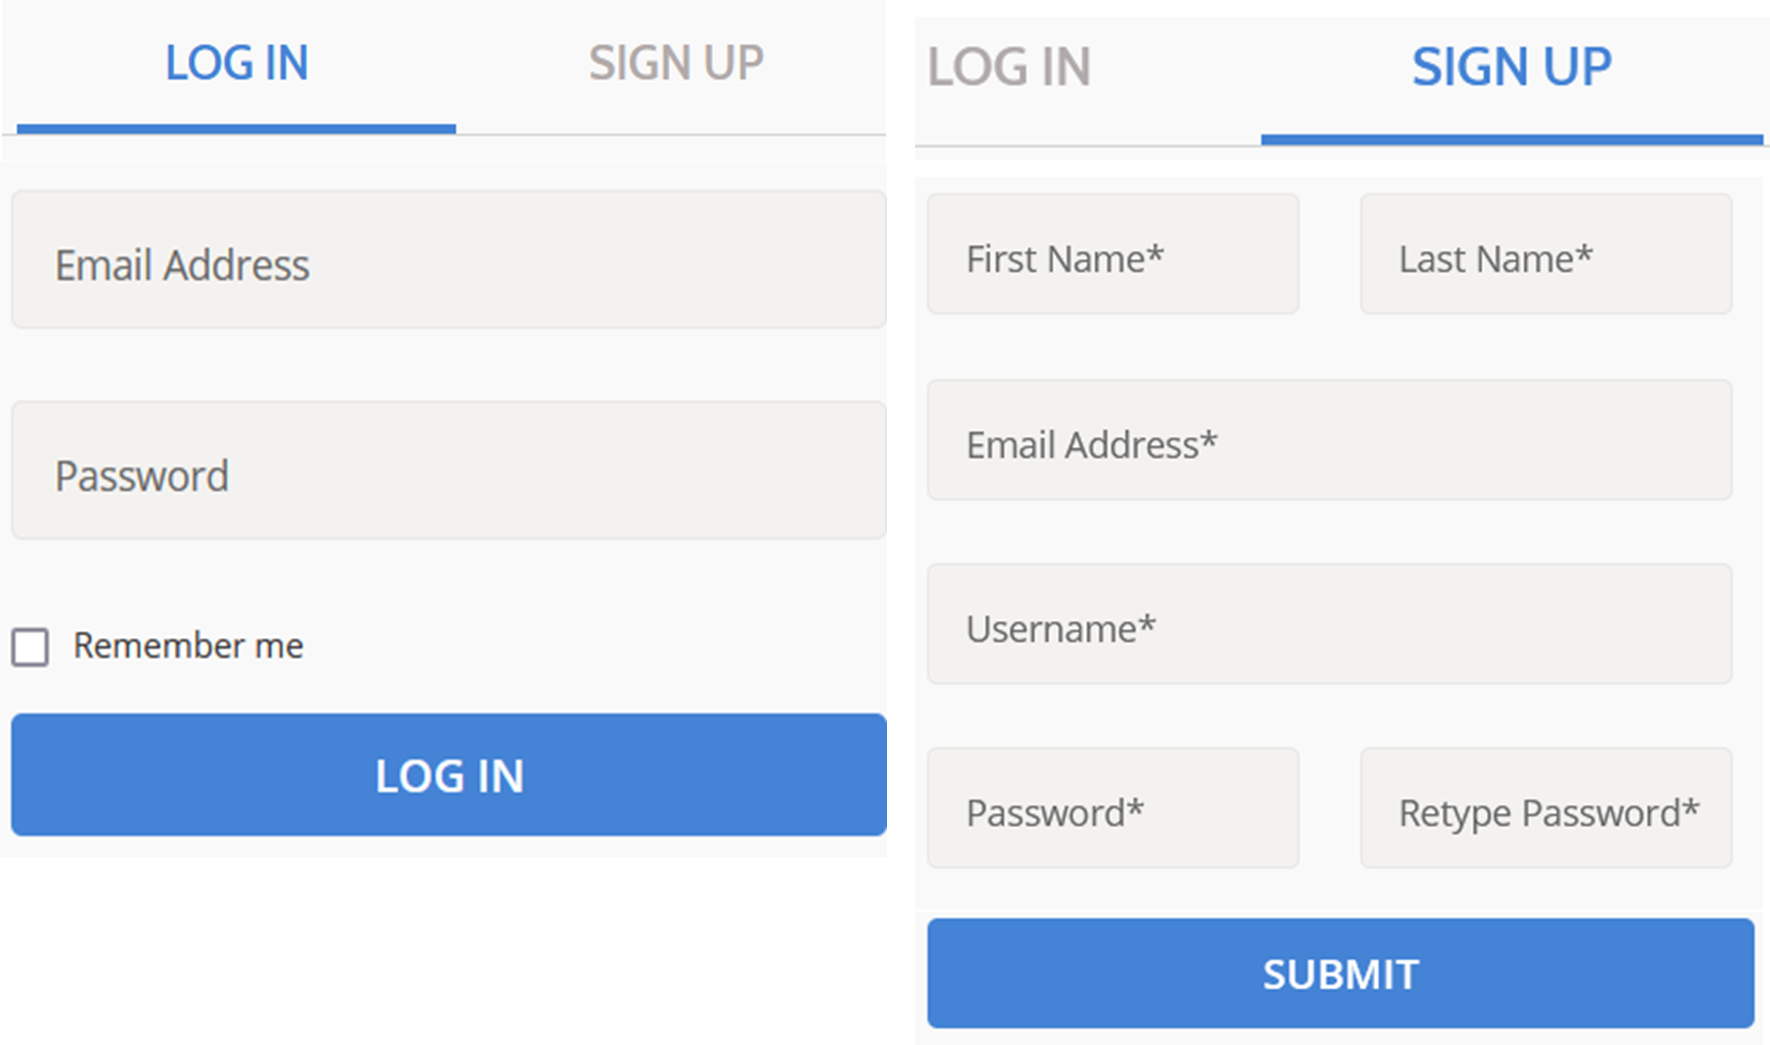
\includegraphics[scale=0.8]{slike/Slika4.PNG} %veličina slike u odnosu na originalnu datoteku i pozicija slike
	\centering
	\caption{Prijava i registracija u sustav}
	\label{fig:promjene4}
\end{figure}

Sustav koriste i moderatori koji su interni zaposlenici projekta, a njihovi računi se dodaju direktno u bazu podataka. Moderatori se prijavljuju u sustav jednako kao i ostali korisnici. Oni mogu dodati komentar na nekome receptu koji će kao i kod autora  biti dodatno vizualno označen, ali ne mogu ocjenjivati recepte.
\newline

Dodatne mogućnosti moderatora su:

\begin{packed_item}
	\item brisanje komentara
	\item brisanje recepata
	\item pregled korisnika sustava.
\end{packed_item}
Također sustav mora biti funkcionalan ukoliko je više korisnika prijavljeno u isto vrijeme neovisno o tome jesu li moderatori ili obični registrirani korisnici.


\eject




\chapter{Specifikacija programske potpore}

\section{Funkcionalni zahtjevi}

\noindent \textbf{Dionici:}

\begin{packed_enum}

	\item Korisnici
	\begin{enumerate}
		\item Registrirani/prijavljeni
		\item Neregistrirani
	\end{enumerate}
	\item Moderator
	\item Razvojni tim

\end{packed_enum}



\noindent \textbf{Aktori i njihovi funkcionalni zahtjevi:}


\begin{packed_enum}
	\item  \underbar{Neregistrirani/neprijavljeni korisnik (inicijator) može:}

	\begin{packed_enum}

		\item Pregledati sve recepte
		\item Sortirati i filtrirati recepte po raznim argumentima
		\item Filtrirati recepte po sastojcima
		\item Pretražiti recepte po imenu/autoru
		\item Registrirati se

	\end{packed_enum}

	\item  \underbar{Registrirani/prijavljeni korisnik (inicijator) može:}

	\begin{packed_enum}

		\item Raditi sve kao i neregistrirani/neprijavljeni korisnik
		\item Dodati vlastiti recept (Dodani recept mora sadržavati maksimalno 5 slika, te po jedan sastojak i korak pripreme)
		\item Urediti vlastiti recept (obrisati/dodati sastojke, urediti i dodati korake i opis)
		\item Dodavati komentare na recepte
		\item Brisati vlastite komentare\newline \newline \newline
	\end{packed_enum}

	\item  \underbar{Moderator (inicijator) ima mogućnost:}

	\begin{packed_enum}

		\item Brisanja i dodavanja komentara, ali ne i ocjenjivanja recepata
		\item Brisanja recepata
		\item Brisanja korisničkih računa
		\item Pregleda svih korisnika
	\end{packed_enum}

	\item  \underbar{Baza podataka (sudionik) mora moći:}

	\begin{packed_enum}

		\item Spremati sve podatke o receptima
		\item Spremati sve podatke o korisnicima
		\item Spremati sve podatke o moderatorima
		\item Izvršiti zadani upit i vratiti rezultat
	\end{packed_enum}
\end{packed_enum}


\eject



\subsection{Obrasci uporabe}

\subsubsection{Opis obrazaca uporabe}

\noindent \underbar{\textbf{UC1 - Sortiranje recepata po popularnosti}}
\begin{packed_item}

	\item \textbf{Glavni sudionik: } Korisnik
	\item  \textbf{Cilj:} Filtrirati recepte po popularnosti
	\item  \textbf{Sudionici:} Baza podataka
	\item  \textbf{Preduvjet:} -
	\item  \textbf{Opis osnovnog tijeka:}

	\item[] \begin{packed_enum}

		\item Prilikom učitavanja je prikazana početna stranica na kojoj se nalazi lista recepata
		\item Korisnik na karti odabire način sortiranja: prema popularnosti
		\item Prikazuju se recepti sortirani silazno prema broju otvaranja

	\end{packed_enum}
\end{packed_item}

\noindent \underbar{\textbf{UC2 - Sortiranje recepata prema prosječnoj ocjeni}}
\begin{packed_item}

	\item \textbf{Glavni sudionik: } Korisnik
	\item  \textbf{Cilj:} Filtrirati recepte prema prosječnoj ocjeni
	\item  \textbf{Sudionici:} Baza podataka
	\item  \textbf{Preduvjet:} -
	\item  \textbf{Opis osnovnog tijeka:}

	\item[] \begin{packed_enum}

		\item Prilikom učitavanja je prikazana početna stranica na kojoj se nalazi lista recepata
		\item Korisnik na karti odabire način sortiranja: prema prosječnoj ocjeni
		\item Prikazuju se recepti sortirani silazno prema prosječnoj ocjeni korisnika

	\end{packed_enum}
\end{packed_item}

\noindent \underbar{\textbf{UC3 - Sortiranje recepata prema oznaci "Preporučeno"}}
\begin{packed_item}

	\item \textbf{Glavni sudionik: } Korisnik
	\item  \textbf{Cilj:} Filtrirati recepte prema oznaci “Preporučeno“
	\item  \textbf{Sudionici:} Baza podataka
	\item  \textbf{Preduvjet:} -
	\item  \textbf{Opis osnovnog tijeka:}

	\item[] \begin{packed_enum}

		\item Prilikom učitavanja je prikazana početna stranica na kojoj se nalazi lista recepata
		\item Korisnik na karti odabire način sortiranja: prema prosječnoj ocjeni
		\item Prikazuju se recepti sortirani silazno prema oznaci “Preporučeno“ koja se određuje kao funkcija popularnosti i ocjene koja je prepuštena projektantima

	\end{packed_enum}
\end{packed_item}

\noindent \underbar{\textbf{UC4 – Pretraživanje recepata po naslovu}}
\begin{packed_item}

	\item \textbf{Glavni sudionik: } Korisnik
	\item  \textbf{Cilj:} Prikazati sve recepte koje sadrže upisani termin
	\item  \textbf{Sudionici:} Baza podataka
	\item  \textbf{Preduvjet:} -
	\item  \textbf{Opis osnovnog tijeka:}

	\item[] \begin{packed_enum}

		\item Prilikom učitavanja je prikazana početna stranica na kojoj se nalazi lista recepata
		\item Korisnik pretražuje određeni termin tako da upiše naslov recepta kojeg želi otvoriti
		\item Prikazuju se svi recepti koji sadrže upisani termin

	\end{packed_enum}
\end{packed_item}

\noindent \underbar{\textbf{UC5 – Pretraživanje recepata po sastojcima}}
\begin{packed_item}

	\item \textbf{Glavni sudionik: } Korisnik
	\item  \textbf{Cilj:} Prikazati sve recepte čiji sastojci su najsličniji unesenim sastojcima
	\item  \textbf{Sudionici:} Baza podataka
	\item  \textbf{Preduvjet:} -
	\item  \textbf{Opis osnovnog tijeka:}

	\item[] \begin{packed_enum}

		\item Prilikom učitavanja je prikazana početna stranica na kojoj se nalazi lista recepata
		\item Korisnik upisuje sastojke koje ima pri ruci
		\item Prikazuju se recepti sortirani po vrijednosti indeksa sličnosti

	\end{packed_enum}
\end{packed_item}

\noindent \underbar{\textbf{UC6 – Registracija}}
\begin{packed_item}

	\item \textbf{Glavni sudionik: } Korisnik
	\item  \textbf{Cilj:} Stvoriti korisnički račun za pristup sustavu
	\item  \textbf{Sudionici:} Baza podataka
	\item  \textbf{Preduvjet:} -
	\item  \textbf{Opis osnovnog tijeka:}

	\item[] \begin{packed_enum}

		\item Korisnik odabire opciju za registraciju
		\item Korisnik unosi potrebne korisničke podatke
		\item Korisnik prima obavijest o uspješnoj registraciji te se podaci spremaju u bazu podataka

	\end{packed_enum}

	\item  \textbf{Opis mogućih odstupanja:}

	\item[] \begin{packed_item}

		\item[2.a] Odabir već zauzetog korisničkog imena i/ili e-maila, unos korisničkog podatka u nedozvoljenom formatu ili pružanje neispravnoga e-maila

		\item[] \begin{packed_enum}

			\item Sustav obavještava korisnika o neuspjelom upisu i vraća ga na stranicu za registraciju
			\item Korisnik mijenja potrebne podatke te završava unos ili odustaje od registracije

		\end{packed_enum}

	\end{packed_item}
\end{packed_item}

\noindent \underbar{\textbf{UC7 – Prijava u sustav}}
\begin{packed_item}

	\item \textbf{Glavni sudionik: } Korisnik
	\item  \textbf{Cilj:} Dobiti pristup dodatnim funkcionalnostima poput unosa, pregledavanja i uređivanja
	\item  \textbf{Sudionici:} Baza podataka
	\item  \textbf{Preduvjet:} Registracija
	\item  \textbf{Opis osnovnog tijeka:}

	\item[] \begin{packed_enum}

		\item Unos korisničkog imena i lozinke
		\item Potvrda o ispravnosti unesenih podataka
		\item Pristup korisničkim funkcijama

	\end{packed_enum}

	\item  \textbf{Opis mogućih odstupanja:}

	\item[] \begin{packed_item}

		\item[1.a] Neispravno korisničko ime ili lozinka

		\item[] \begin{packed_enum}

			\item Sustav obavještava korisnika o neuspjelom upisu i omogućuje mu ponovno prijavu u sustav

		\end{packed_enum}

	\end{packed_item}
\end{packed_item}

\noindent \underbar{\textbf{UC8 – Pregled pojedinog recepta}}
\begin{packed_item}

	\item \textbf{Glavni sudionik: } Korisnik
	\item  \textbf{Cilj:} Prikazati sve podatke vezane za recept
	\item  \textbf{Sudionici:} Baza podataka
	\item  \textbf{Preduvjet:} -
	\item  \textbf{Opis osnovnog tijeka:}

	\item[] \begin{packed_enum}

		\item Korisnik odabere jedan od ponuđenih recepata
		\item Otvori se stranica sa svim informacijama o receptu \newline \newline \newline
	\end{packed_enum}
\end{packed_item}

\noindent \underbar{\textbf{UC9 – Komentiranje i ocjenjivanje recepata}}
\begin{packed_item}

	\item \textbf{Glavni sudionik: } Korisnik
	\item  \textbf{Cilj:} Ostaviti komentar i ocjenu za određeni recept
	\item  \textbf{Sudionici:} Baza podataka
	\item  \textbf{Preduvjet:} Korisnik je prijavljen
	\item  \textbf{Opis osnovnog tijeka:}

	\item[] \begin{packed_enum}

		\item Korisnik napiše recenziju i ocijeni recept
		\item Ocjena i osvrt se pohranjuju u bazu podataka i ažurira se prosječna ocjena recepta
	\end{packed_enum}
\end{packed_item}

\noindent \underbar{\textbf{UC10 – Pregled svih recepata određenog autora}}
\begin{packed_item}

	\item \textbf{Glavni sudionik: } Korisnik
	\item  \textbf{Cilj:} Prikazati sve recepte određenog autora
	\item  \textbf{Sudionici:} Baza podataka
	\item  \textbf{Preduvjet:} Korisnik mora biti na stranici recepta
	\item  \textbf{Opis osnovnog tijeka:}

	\item[] \begin{packed_enum}

		\item Korisnik se nalazi na stranici recepta
		\item Korisnik odabire opciju “Prikaži sve recepte autora“
		\item Prikazuju se svi recepti autora uključujući i odabrani recept
	\end{packed_enum}
\end{packed_item}

\noindent \underbar{\textbf{UC11 – Dodavanje recepta}}
\begin{packed_item}

	\item \textbf{Glavni sudionik: } Korisnik
	\item  \textbf{Cilj:} Dodati novi recept
	\item  \textbf{Sudionici:} Baza podataka
	\item  \textbf{Preduvjet:} Korisnik je prijavljen
	\item  \textbf{Opis osnovnog tijeka:}

	\item[] \begin{packed_enum}

		\item Korisnik odabire opciju za dodavanje novog recepta
		\item Korisnik prilaže maksimalno 5 slika jela, sastojke (makar 1) i količinu te korake pripreme (makar 1)
		\item Ukoliko je korisnik zadovoljio uvjete, podaci se spremaju u bazu podataka te su vidljivi u aplikaciji
	\end{packed_enum}

	\item  \textbf{Opis mogućih odstupanja:}

	\item[] \begin{packed_item}

		\item[2.a] Korisnik nije priložio niti jedan sastojak ili jedan korak pripreme

		\item[] \begin{packed_enum}

			\item Sustav obavještava korisnika o uvjetima koji nisu zadovoljeni
			\item Korisnik dodaje potrebne podatke te završava unos ili odustaje od dodavanja recepta

		\end{packed_enum}

	\end{packed_item}
\end{packed_item}

\noindent \underbar{\textbf{UC12 – pregled vlastitih recepata}}
\begin{packed_item}

	\item \textbf{Glavni sudionik: } Korisnik
	\item  \textbf{Cilj:} Prikazati sve vlastite recepte
	\item  \textbf{Sudionici:} Baza podataka
	\item  \textbf{Preduvjet:} Korisnik mora biti prijavljen
	\item  \textbf{Opis osnovnog tijeka:}

	\item[] \begin{packed_enum}

		\item Korisnik odabire opciju “Pregledaj recepte“
		\item Korisniku se prikazuju svi recepti kojima je on autor
	\end{packed_enum}
\end{packed_item}

\noindent \underbar{\textbf{UC13 – Uređivanje recepta}}
\begin{packed_item}

	\item \textbf{Glavni sudionik: } Korisnik
	\item  \textbf{Cilj:} Urediti željeni recept
	\item  \textbf{Sudionici:} Baza podataka
	\item  \textbf{Preduvjet:} Korisnik je autor recepta
	\item  \textbf{Opis osnovnog tijeka:}

	\item[] \begin{packed_enum}

		\item Korisnik odabire opciju uređivanja recepta
		\item Korisnik unosi željene podatke
		\item Ukoliko su uvjeti zadovoljeni, korisnik prima obavijest o uspješnom uređivanju recepta
	\end{packed_enum}

	\item  \textbf{Opis mogućih odstupanja:}

	\item[] \begin{packed_item}

		\item[2.a] Korisnik je prilikom uređivanja uklonio sve sastojke ili korake pripreme

		\item[] \begin{packed_enum}

			\item Sustav obavještava korisnika o uvjetima koji nisu zadovoljeni
			\item Korisnik dodaje potrebne podatke te završava izmjene ili odustaje od uređivanja recepta te recept ostaje nepromijenjen

		\end{packed_enum}

	\end{packed_item}
\end{packed_item}

\noindent \underbar{\textbf{UC14 – Dodavanje komentara moderatora}}
\begin{packed_item}

	\item \textbf{Glavni sudionik: } Korisnik
	\item  \textbf{Cilj:} Dodati komentar na određeni recept
	\item  \textbf{Sudionici:} Baza podataka
	\item  \textbf{Preduvjet:} Moderator mora biti prijavljen
	\item  \textbf{Opis osnovnog tijeka:}

	\item[] \begin{packed_enum}

		\item Moderator ostavlja komentar koji je u konačnici vizualno dodatno naglašen
		\item Komentar se pohranjuje u bazu podataka \newline
	\end{packed_enum}
\end{packed_item}

\noindent \underbar{\textbf{UC15 – Brisanje komentara}}
\begin{packed_item}

	\item \textbf{Glavni sudionik: } Korisnik
	\item  \textbf{Cilj:} Obrisati komentare koji nisu primijenjeni
	\item  \textbf{Sudionici:} Baza podataka
	\item  \textbf{Preduvjet:} Moderator mora biti prijavljen
	\item  \textbf{Opis osnovnog tijeka:}

	\item[] \begin{packed_enum}

		\item Moderator odabire željeni komentar za određeni recept
		\item Klikom na komentar prikaže mu se opcija “Izbriši“
		\item Komentar se uklanja iz baze podataka
	\end{packed_enum}
\end{packed_item}

\noindent \underbar{\textbf{UC16 – Brisanje vlastitih komentara}}
\begin{packed_item}

	\item \textbf{Glavni sudionik: } Korisnik
	\item  \textbf{Cilj:} Autor želi izbrisati svoj komentar
	\item  \textbf{Sudionici:} Baza podataka
	\item  \textbf{Preduvjet:} Korisnik mora biti prijavljen
	\item  \textbf{Opis osnovnog tijeka:}

	\item[] \begin{packed_enum}

		\item Korisnik na stranici recepta odabire vlastiti komentar
		\item Klikom na komentar prikaže mu se opcija “Izbriši“
		\item Komentar se uklanja iz baze podataka
	\end{packed_enum}
\end{packed_item}

\noindent \underbar{\textbf{UC17 - Brisanje recepata}}
\begin{packed_item}

	\item \textbf{Glavni sudionik: } Moderator
	\item  \textbf{Cilj:} Obrisati željene recepte
	\item  \textbf{Sudionici:} Baza podataka
	\item  \textbf{Preduvjet:} Moderator mora biti prijavljen
	\item  \textbf{Opis osnovnog tijeka:}

	\item[] \begin{packed_enum}

		\item Moderator odabire željeni recept
		\item Klikom na opciju “Izbriši“ recept se uklanja iz baze podataka
	\end{packed_enum}
\end{packed_item}

\noindent \underbar{\textbf{UC18 - Brisanje vlastitih recepata}}
\begin{packed_item}

	\item \textbf{Glavni sudionik: } Korisnik
	\item  \textbf{Cilj:} Autor želi obrisati svoj recept
	\item  \textbf{Sudionici:} Baza podataka
	\item  \textbf{Preduvjet:} Korisnik mora biti prijavljen
	\item  \textbf{Opis osnovnog tijeka:}

	\item[] \begin{packed_enum}

		\item Korisnik odabire recept kojemu je on autor
		\item Klikom na opciju “Izbriši“ recept se uklanja iz baze podataka
	\end{packed_enum}
\end{packed_item}

\noindent \underbar{\textbf{UC19 - Pregled korisnika sustava}}
\begin{packed_item}

	\item \textbf{Glavni sudionik: } Moderator
	\item  \textbf{Cilj:} Pregledati registrirane korisnike
	\item  \textbf{Sudionici:} Baza podataka
	\item  \textbf{Preduvjet:} Moderator mora biti prijavljen
	\item  \textbf{Opis osnovnog tijeka:}

	\item[] \begin{packed_enum}

		\item Moderator odabire opciju pregledavanja korisnika
		\item Prikaže se lista svih ispravno registriranih korisnika s osobnim podacima
	\end{packed_enum}
\end{packed_item}

\noindent \underbar{\textbf{UC20 - Brisanje korisnika}}
\begin{packed_item}

	\item \textbf{Glavni sudionik: } Moderator
	\item  \textbf{Cilj:} Obrisati korisnika
	\item  \textbf{Sudionici:} Baza podataka
	\item  \textbf{Preduvjet:} Moderator mora biti prijavljen
	\item  \textbf{Opis osnovnog tijeka:}

	\item[] \begin{packed_enum}

		\item Moderator odabire opciju uklanjanja korisnika
		\item Moderator pronalazi željenog korisnika
		\item Moderator uklanja željenog korisnika i njegove podatke iz baze podataka \newline \newline \newline \newline \newline \newline \newline \newline \newline \newline \newline \newline
	\end{packed_enum}
\end{packed_item}

\subsubsection{Dijagrami obrazaca uporabe}

\begin{figure}[H]
	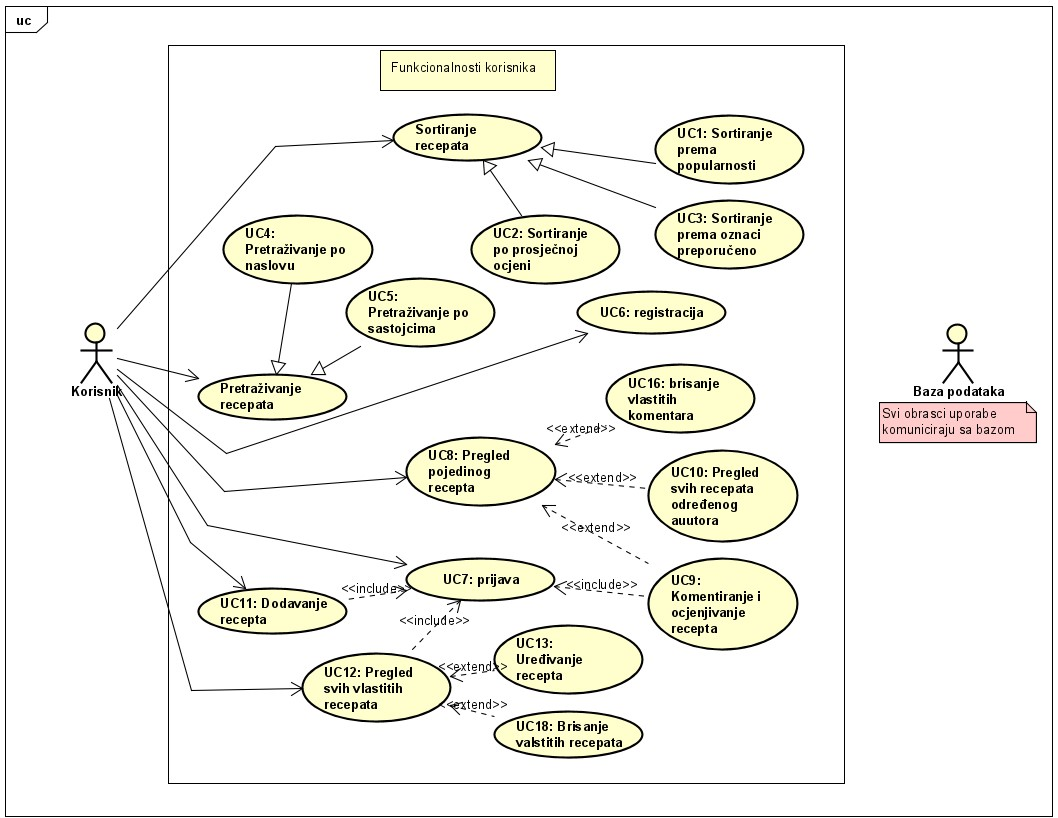
\includegraphics[scale=0.8]{slike/Slika5.jpg} %veličina slike u odnosu na originalnu datoteku i pozicija slike
	\centering
	\caption{Dijagram obrasca uporabe, funkcionalnost korisnika}
	\label{fig:promjene}
\end{figure}

\begin{figure}[H]
	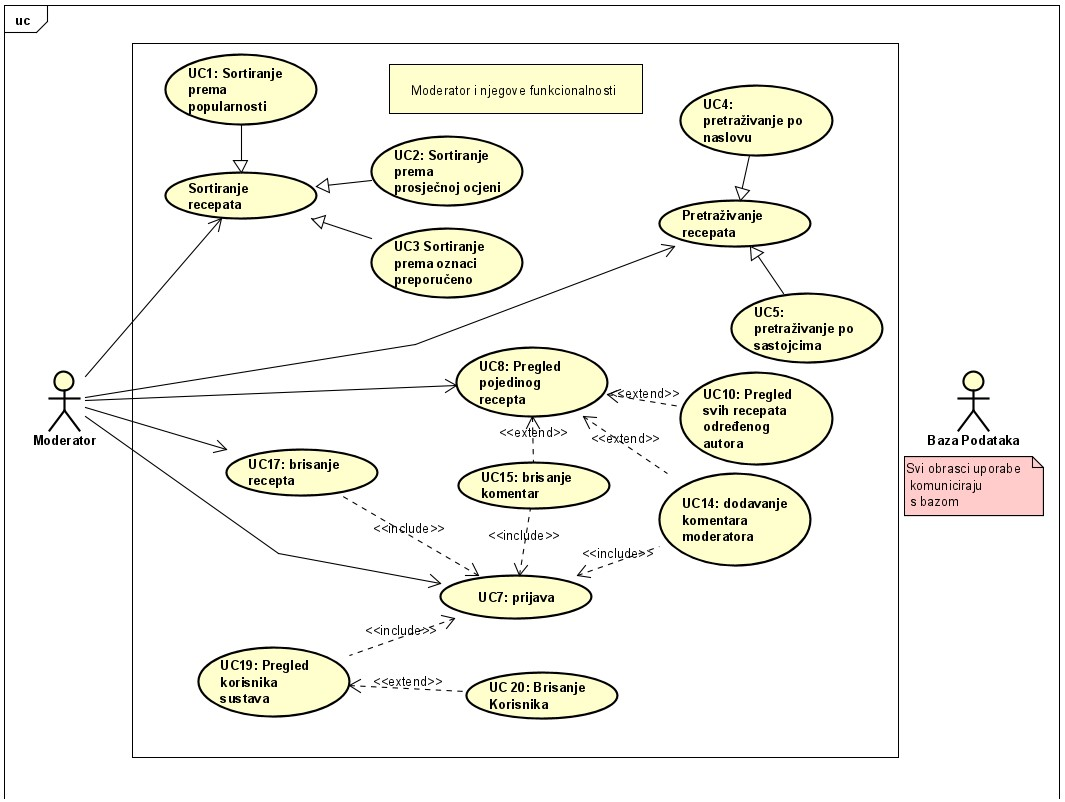
\includegraphics[scale=0.8]{slike/Slika6.jpg} %veličina slike u odnosu na originalnu datoteku i pozicija slike
	\centering
	\caption{Dijagram obrasca uporabe, funkcionalnost moderatora}
	\label{fig:promjene}
\end{figure}

\eject

\subsection{Sekvencijski dijagrami}


\noindent\textbf{Obrazac uporabe UC4 - Pretraživanje recepata po naslovu}\\\\
Klijent na početnoj stranici ima uvid u sve recepte, ali ima i mogućnost filtriranja tih recepata.
Jedno od mogućnosti filtriranja jest filtriranje recepata po naslovu.
Klijent upisuje naslov ili dio naslova kojim želi naći određeni recept te pritišće tipku pretraži.
Pritiskom na tipku, web-apliakcija šalje upit bazi podataka.
Baza podataka pretražuje sve recepte i traži one recepte koji imaju sve riječi ili samo jednu riječ upisanu u tražilicu.
Ukoliko baza podataka ne pronađe niti jedan recept nakon pretraživanja, klijent će biti obaviješten o tome.
U suprotnome, baza podataka vraća web-aplikaciji sve recepte koje je pronašla nakon pretraživanja.
Web-apliakcija potom ispisuje sve recepte klijentu te se time završava pretraživanje.
\begin{figure}[H]
	\includegraphics[scale=0.8]{slike/Slika7.png} %veličina slike u odnosu na originalnu datoteku i pozicija slike
	\centering
	\caption{Sekvencijski dijagram za UC4}
	\label{fig:promjene}
\end{figure}
\pagebreak


\noindent\textbf{Obrazac uporabe UC6 - Registracija}\\\\
Klijent ima mogućnost registracije. Registracija je postupak stvaranja računa po prvi puta u web-aplikaciji.
Klijent pritiskom na gumb "prijava" otvara novu web-stranicu gdje mu je omogućena prijava.
Osim prijave, klijentu je omogućena i registracija, ukoliko nema već postojeći račun.
Klikom na registraciju, pojavljuje se obrazac za stvaranje računa gdje je potrebno unijeti podatke koji će se potom spremati u bazu podataka.
Kako bi obrazac bio uspješno napisan potrebno je: ispuniti sva polja, upisati nepostojeće korisničko ime i lozinku koja se pridržava propisanih pravila.
Ako je klijent uspješno ispunio zahtjev, njegov račun će se spremiti u bazu podataka i dobit će obavijest o uspješnoj registraciji.
Ako klijent nije uspješno ispunio zahtjev, dobit će poruku o odgovarajućoj pogrešci.
\begin{figure}[H]
	\includegraphics[scale=1.0]{slike/Slika8.png} %veličina slike u odnosu na originalnu datoteku i pozicija slike
	\centering
	\caption{Sekvencijski dijagram za UC6}
	\label{fig:promjene}
\end{figure}
\pagebreak

\noindent\textbf{Obrazac uporabe UC11 - Dodavanje recepta}\\\\
Registrirani korisnik (nadalje klijent) ima mogućnost dodavanja recepta.
Dodavanje recepta je vidljivo na profilu klijenta.
Odabirom usluge dodavanja recepta, otvara se web-stranica sa obrascem za dodavanje recepta.
U obrascu je potrebno popuniti označena polja, te priložiti do maksimalno 5 slika.
Ako je klijent uspješno popunio obrazac, recept se dodaje u bazu podataka i klijent dobiva obavijest o uspješnome dodavanju recepta.
Ako klijent nije uspješno popunio obrazac, ispisuje mu se odgovarajuća pogreška, ali se postojeći podaci ne brišu te klijent ima mogućnost ispravljanja pogreške.
\begin{figure}[H]
	\includegraphics[scale=0.8]{slike/Slika9.png} %veličina slike u odnosu na originalnu datoteku i pozicija slike
	\centering
	\caption{Sekvencijski dijagram za UC11}
	\label{fig:promjene}
\end{figure}
\pagebreak

\noindent\textbf{Obrazac uporabe UC13 - Uređivanje recepta}\\\\
Registrirani korisnik (nadalje klijent) ima mogućnost uređivanja vlastitog recepta.
Uređivanje recepta je vidljivo na stranici klijentovog recepta.
Odabirom usluge uređivanja recepta, otvara se web-stranica s već postojećim obrascem.
Podaci u već postojećem obrascu izvučeni su iz baze podataka.
Klijent može dodavati ili brisati podatke u obrascu.
Klijent mora poštovati pravila za uređivanje obrasca kao i kod dodavanja recepta.
Ako je klijent napravio prihvatljivu promjenu, promjena će se spremiti u bazu podataka i klijent dobiva obavijest o uspješnome uređivanju recepta.
Ako je klijent napravio neprihvatljivu promjenu, promjena neće biti spremljena i klijent će dobiti obavijest o pogrešci.
\begin{figure}[H]
	\includegraphics[scale=0.8]{slike/Slika10.png} %veličina slike u odnosu na originalnu datoteku i pozicija slike
	\centering
	\caption{Sekvencijski dijagram za UC13}
	\label{fig:promjene}
\end{figure}
\pagebreak

% \textbf{\textit{dio 1. revizije}}\\

% \textit{Nacrtati sekvencijske dijagrame koji modeliraju najvažnije dijelove sustava (max. 4 dijagrama). Ukoliko postoji nedoumica oko odabira, razjasniti s asistentom. Uz svaki dijagram napisati detaljni opis dijagrama.}
\eject

\section{Ostali zahtjevi}


\textit{
	\begin{packed_item}
		\item Sustav treba omogućiti rad više korisnika u stvarnom vremenu
		\item Korisničko sučelje i sustav moraju podržavati hrvatsku abecedu (dijakritičke
		znakove) pri unosu i prikazu tekstualnog sadržaja
		\item Izvršavanje dijela programa u kojem se pristupa bazi podataka ne smije trajati duže od nekoliko sekundi
		\item Sustav treba biti implementiran kao web aplikacija koristeći objektno-orijentirane jezike
		\item Neispravno korištenje korisničkog sučelja ne smije narušiti funkcionalnost i rad sustava
		\item Sustav treba biti jednostavan za korištenje, korisnici se moraju znati koristiti sučeljem bez opširnih uputa
		\item Nadogradnja sustava ne smije narušavati postojeće funkcionalnosti sustava
		\item Veza s bazom podataka mora biti kvalitetno zaštićena, brza i otporna na vanjske greške
		\item Pristup sustavu mora biti omogućen iz javne mreže pomoću HTTPS.
	\end{packed_item}
}




\chapter{Arhitektura i dizajn sustava}

Arhitektura se može podijeliti na tri podsustava:

\begin{packed_item}
	\item Web poslužitelj
	\item Web aplikacija
	\item Baza podataka
\end{packed_item}

\begin{figure}[H]
	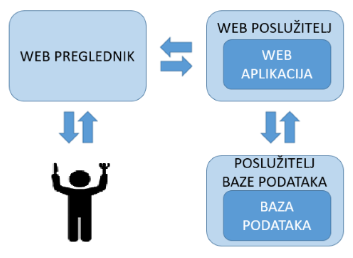
\includegraphics[scale=0.8]{slike/Slika11.png} %veličina slike u odnosu na originalnu datoteku i pozicija slike
	\centering
	\caption{Arhitektura sustava}
	\label{fig:promjene}
\end{figure}

\underline{Web preglednik} je program koji korisniku omogućuje pregled web-stranica i multimedijalnih sadržaja
vezanih uz njih. Svaki internetski preglednik je prevoditelj. Dakle, stranica je pisana u kodu koji
preglednik nakon toga interpretira kao nešto svakome razumljivo. Korisnik putem web preglednika šalje
zahtjev web poslužitelju.
\newline \underline{Web poslužitelj} osnova je rada web aplikacije. Njegova primarna zadaća je komunikacija klijenta s aplikacijom.
Komunikacija se odvija preko HTTP (engl. Hyper Text Transfer Protocol) protokola, što je protokol u prijenosu
informacija na webu. Poslužitelj je onaj koji pokreće web aplikaciju te joj prosljeđuje zahtjev. \newline Korisnik koristi
\underline{web aplikaciju} za obrađivanje željenih zahtjeva. Web aplikacija obrađuje zahtjev te ovisno o zahtjevu, pristupa
bazi podataka nakon čega preko poslužitelja vraća korisniku odgovor u obliku HTML dokumenta vidljivog u web pregledniku. \newline
\newline Programski jezik kojeg smo odabrali za izradu naše web aplikacije je Java zajedno sa Spring Boot radnim okvirom. Odabrano razvojno okruženje je Visual Studio Code.
Arhitektura sustava temeljiti će se na MVC (Model-View-Controller) konceptu. \newline
Karakteristika MVC koncepta je nezavisan razvoj pojedinih dijelova aplikacije što za posljedicu ima jednostavnije
ispitivanje kao i jednostavno razvijanje i dodavanje novih svojstava u sustav.\newline MVC koncept sastoji se od:
\begin{packed_item}
	\item \textbf{Model} - Središnja komponenta sustava. Predstavlja dinamičke strukture podataka, neovisne
	o korisničkom sučelju. Izravno upravlja podacima, logikom i pravilima aplikacije. Također prima ulazne podatke od Controllera.
	\item \textbf{View} - Bilo kakav prikaz podataka, poput grafa. Mogući su različiti prikazi iste informacije poput
	grafičkog ili tabličnog prikaza podataka.
	\item \textbf{Controller} - Prima ulaze i prilagođava ih za prosljeđivanje Modelu ili Viewu. Upravlja
	korisničkim zahtjevima i temeljem njih izvodi daljnju interakciju s ostalim elementima sustava.
\end{packed_item}

\newpage



\section{Baza podataka}

Za potrebe našeg sustava koristit ćemo relacijsku bazu podataka koja svojom strukturom olakšava modeliranje stvarnog svijeta. Gradivna jedinka baze je relacija,
odnosno tablica koja je definirana svojim imenom i skupom atributa. Zadaća baze podataka je brza i jednostavna
pohrana, izmjena i dohvat podataka za daljnju obradu. Baza podataka ove aplikacije sastoji se od sljedećih entiteta:

\begin{packed_item}
	\item Users
	\item Roles
	\item Images
	\item Ingredients
	\item Recipes
	\item Ratings
	\item \texttt{Recipe\_steps}

\end{packed_item}

\subsection{Opis tablica}

\textbf{Users}  Ovaj entitet sadržava sve važne informacije o korisniku aplikacije.
Sadrži atribute: \texttt{first\_name}, \texttt{last\_name}, \texttt{date\_of\_birth}, \texttt{email}, \texttt{id}, \texttt{password\_hash}, \texttt{username} \texttt{role\_id}. Ovaj entitet u vezi
je \textit{Many-to-One} s entitetom Roles preko atributa \texttt{role\_id}, u vezi \textit{One-to-Many}
s entitetom Recipes preko atributa \texttt{created\_by} te je u vezi \textit{One-to-Many} s entitetom Ratings
preko atributa \texttt{user\_id}.

\begin{longtblr}[
	label=none,
	entry=none
	]{
	width = \textwidth,
	colspec={|X[7,l]|X[6, l]|X[20, l]|},
	rowhead = 1,
	} %definicija širine tablice, širine stupaca, poravnanje i broja redaka naslova tablice
	\hline \multicolumn{3}{|c|}{\textbf{Users}}	 \\ \hline[3pt]
	\SetCell{LightGreen} \texttt{id} & SERIAL	&  	jedinstveni identifikator korisnika  	\\ \hline
	\texttt{first\_name}	& VARCHAR &  ime korisnika 	\\ \hline
	\texttt{last\_name} & VARCHAR & prezime korisnika \\ \hline
	\texttt{date\_of\_birth} & DATE	& datum rođenja korisnika 	\\ \hline
	\texttt{email} & VARCHAR	& korisnikov email 	\\ \hline
	\texttt{password\_hash} & VARCHAR	& korisnikova lozinka 	\\ \hline
	\texttt{username} & VARCHAR	& korisničko ime 	\\ \hline
	\SetCell{LightBlue} \texttt{role\_id}	& INT & strani ključ na entitet Roles	\\ \hline
\end{longtblr}

\newpage

\textbf{Recipes}  Ovaj entitet sadržava sve važne informacije o receptu unutar aplikacije.
Sadrži atribute: \texttt{id}, \texttt{popularity}, \texttt{title}, \texttt{created\_at},
\texttt{last\_updated\_at}, \texttt{recipe\_description}, \texttt{estimated\_time} i \texttt{created\_by}.
Ovaj entitet u vezi je \textit{One-to-Many} s entitetom Ingredients preko atributa \texttt{recipe\_id},
u vezi \textit{One-to-Many} s entitetom Images preko atributa \texttt{recipe\_id}, u vezi \textit{Many-to-One}
s entitetom Users preko atributa \texttt{created\_by}, u vezi \textit{One-to-Many} s entitetom Ratings preko atributa
\texttt{recipe\_id} te je u vezi \textit{One-to-Many} s entitetom \texttt{Recipe\_steps} preko atributa
\texttt{recipe\_id}.

\begin{longtblr}[
	label=none,
	entry=none
	]{
	width = \textwidth,
	colspec={|X[10,l]|X[6, l]|X[20, l]|},
	rowhead = 1,
	} %definicija širine tablice, širine stupaca, poravnanje i broja redaka naslova tablice
	\hline \multicolumn{3}{|c|}{\textbf{Recipes}}	 \\ \hline[3pt]
	\SetCell{LightGreen} \texttt{id} & SERIAL	&  	jedinstveni identifikator recepta  	\\ \hline
	\texttt{popularity}	& INT &  popularnost recepta 	\\ \hline
	\texttt{title} & VARCHAR & naslov recepta \\ \hline
	\texttt{created\_at} & TIMESTAMP	& datum nastanka recepta 	\\ \hline
	\texttt{last\_updated\_at} & TIMESTAMP	& datum zadnje izmjene recepta 	\\ \hline
	\texttt{recipe\_description} & VARCHAR	& kratki opis recepta 	\\ \hline
	\texttt{estimated\_time} & INT	& procijenjeno vrijeme za pripremu  	\\ \hline
	\SetCell{LightBlue} \texttt{created\_by}	& INT & strani ključ na entitet Users	\\ \hline
\end{longtblr}

\textbf{Ingredients}  Ovaj entitet predstavlja jedan sastojak unutar nekog recepta.
Sadrži atribute: \texttt{id}, \texttt{ingredient\_name}, \texttt{ingredient\_measure},
\texttt{ingredient\_quantity} i \texttt{ingredient\_order}.
Ovaj entitet u vezi je \textit{Many-to-One} s entitetom Recipes preko atributa \texttt{recipe\_id}.

\begin{longtblr}[
	label=none,
	entry=none
	]{
	width = \textwidth,
	colspec={|X[11,l]|X[6, l]|X[20, l]|},
	rowhead = 1,
	} %definicija širine tablice, širine stupaca, poravnanje i broja redaka naslova tablice
	\hline \multicolumn{3}{|c|}{\textbf{Ingredients}}	 \\ \hline[3pt]
	\SetCell{LightGreen} \texttt{id} & SERIAL	&  	jedinstveni identifikator sastojka  	\\ \hline
	\texttt{ingredient\_name}	& VARCHAR &  ime sastojka 	\\ \hline
	\texttt{ingredient\_quantity} & INT & količina sastojka \\ \hline
	\texttt{ingredient\_measure} & VARCHAR	& ime mjere sastojka(ml, g, kg) 	\\ \hline
	\texttt{ingredient\_order} & INT	& redni broj sastojka unutar recepta  	\\ \hline
	\SetCell{LightBlue} \texttt{recipe\_id}	& INT & strani ključ na entitet Recipes	\\ \hline
\end{longtblr}

\textbf{Ratings}  Ovaj entitet predstavlja ocjenu na određeni recept.
Sadrži atribute: \texttt{id}, \texttt{rating\_value}, \texttt{user\_id} i \texttt{recipe\_id}.
Ovaj entitet u vezi je \textit{Many-to-One} s entitetom Recipes preko atributa \texttt{recipe\_id}
te je u vezi \textit{Many-to-One} s entitetom Users preko atributa \texttt{user\_id}

\begin{longtblr}[
	label=none,
	entry=none
	]{
	width = \textwidth,
	colspec={|X[10,l]|X[6, l]|X[20, l]|},
	rowhead = 1,
	} %definicija širine tablice, širine stupaca, poravnanje i broja redaka naslova tablice
	\hline \multicolumn{3}{|c|}{\textbf{Ratings}}	 \\ \hline[3pt]
	\SetCell{LightGreen} \texttt{id} & SERIAL	&  	jedinstveni identifikator ocjene  	\\ \hline
	\texttt{rating\_value}	& INT &  vrijednost ocjene 	\\ \hline
	\SetCell{LightBlue} \texttt{user\_id}	& INT & strani ključ na entitet Users	\\ \hline
	\SetCell{LightBlue} \texttt{recipe\_id}	& INT & strani ključ na entitet Recipes	\\ \hline
\end{longtblr}

\textbf{Images}  Ovaj entitet predstavlja jednu sliku koja se dodaje prilikom dodavanja recepta.
Sadrži atribute: \texttt{id}, \texttt{image\_data}, \texttt{image\_order} i \texttt{recipe\_id}.
Ovaj entitet u vezi je \textit{Many-to-One} s entitetom Recipes preko atributa \texttt{recipe\_id}.

\begin{longtblr}[
	label=none,
	entry=none
	]{
	width = \textwidth,
	colspec={|X[10,l]|X[6, l]|X[20, l]|},
	rowhead = 1,
	} %definicija širine tablice, širine stupaca, poravnanje i broja redaka naslova tablice
	\hline \multicolumn{3}{|c|}{\textbf{Images}}	 \\ \hline[3pt]
	\SetCell{LightGreen} \texttt{id} & SERIAL	&  	jedinstveni identifikator slike  	\\ \hline
	\texttt{image\_data}	& BYTEA &  prostor koji zauzima slika u memoriji 	\\ \hline
	\texttt{image\_order}	& INT &  poredak slike prilikom dodavanja 	\\ \hline
	\SetCell{LightBlue} \texttt{recipe\_id}	& INT & strani ključ na entitet Recipes	\\ \hline
\end{longtblr}

\textbf{\texttt{Recipe\_steps}}  Ovaj entitet predstavlja jedan korak pripreme u receptu.
Sadrži atribute: \texttt{id}, \texttt{step\_order}, \texttt{step\_description} i \texttt{recipe\_id}.
Ovaj entitet u vezi je \textit{Many-to-One} s entitetom Recipes preko atributa \texttt{recipe\_id}.

\begin{longtblr}[
	label=none,
	entry=none
	]{
	width = \textwidth,
	colspec={|X[10,l]|X[6, l]|X[20, l]|},
	rowhead = 1,
	} %definicija širine tablice, širine stupaca, poravnanje i broja redaka naslova tablice
	\hline \multicolumn{3}{|c|}{\textbf{\texttt{Recipe\_steps}}}	 \\ \hline[3pt]
	\SetCell{LightGreen} \texttt{id} & SERIAL	&  	jedinstveni identifikator koraka pripreme  	\\ \hline
	\texttt{step\_order}	& INT &  redni broj koraka pripreme 	\\ \hline
	\texttt{step\_description}	& VARCHAR &  kratki opis koraka pripreme 	\\ \hline
	\SetCell{LightBlue} \texttt{recipe\_id}	& INT & strani ključ na entitet Recipes	\\ \hline
\end{longtblr}

\textbf{Roles}  Ovaj entitet predstavlja ulogu korisnika u sustavu.
Sadrži atribute: \texttt{id} i \texttt{role\_name}.
Ovaj entitet u vezi je \textit{One-to-Many} s entitetom Users preko atributa \texttt{role\_id}.

\begin{longtblr}[
	label=none,
	entry=none
	]{
	width = \textwidth,
	colspec={|X[10,l]|X[6, l]|X[20, l]|},
	rowhead = 1,
	} %definicija širine tablice, širine stupaca, poravnanje i broja redaka naslova tablice
	\hline \multicolumn{3}{|c|}{\textbf{Roles}}	 \\ \hline[3pt]
	\SetCell{LightGreen} \texttt{id} & SERIAL	&  	jedinstveni identifikator uloge  	\\ \hline
	\texttt{role\_name}	& VARCHAR &  ime uloge (korisnik, moderator) 	\\ \hline
\end{longtblr}

\newpage

\subsection{Dijagram baze podataka}


\begin{figure}[H]
	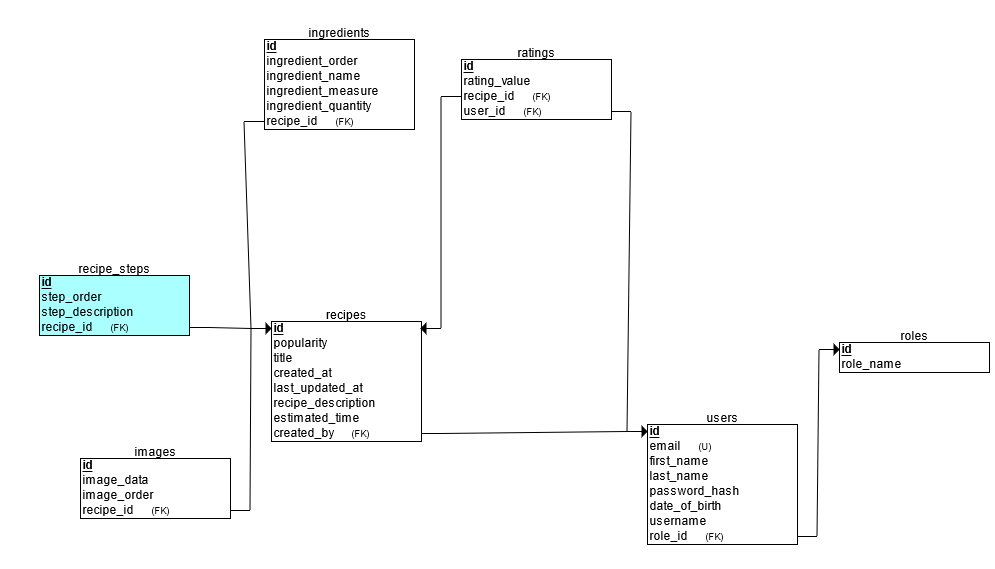
\includegraphics[scale=0.65]{slike/Slika12.png} %veličina slike u odnosu na originalnu datoteku i pozicija slike
	\centering
	\caption{E-R dijagram baze podataka}
	\label{fig:promjene}
\end{figure}


\eject


\section{Dijagram razreda}
Na slikama 4.3, 4.4 i 4.5 prikazani su razredi koji pripadaju backend dijelu MVC arhitekture. Razredi prikazani na 4.3 su Model razredi koji su implementacije entiteta baze. Razredi prikazani na slici 4.3 su Controller razredi te oni implementiraju funkcionalnosti u ovisnosti na HTTP upit i vraćaju valjani odgovor u JSON formatu. Bazi se pristupa preko Interfacea koji nasljeđuju JpaRepository. \\

Zbog lakše organizacije razredi su podijeljeni na tri logičke jedinice te su prikazani odvojenim dijagramima. Iz naziva i tipova atributa mogu se zaključiti ostale ovisnosti među razredima.

\begin{figure}[H]
	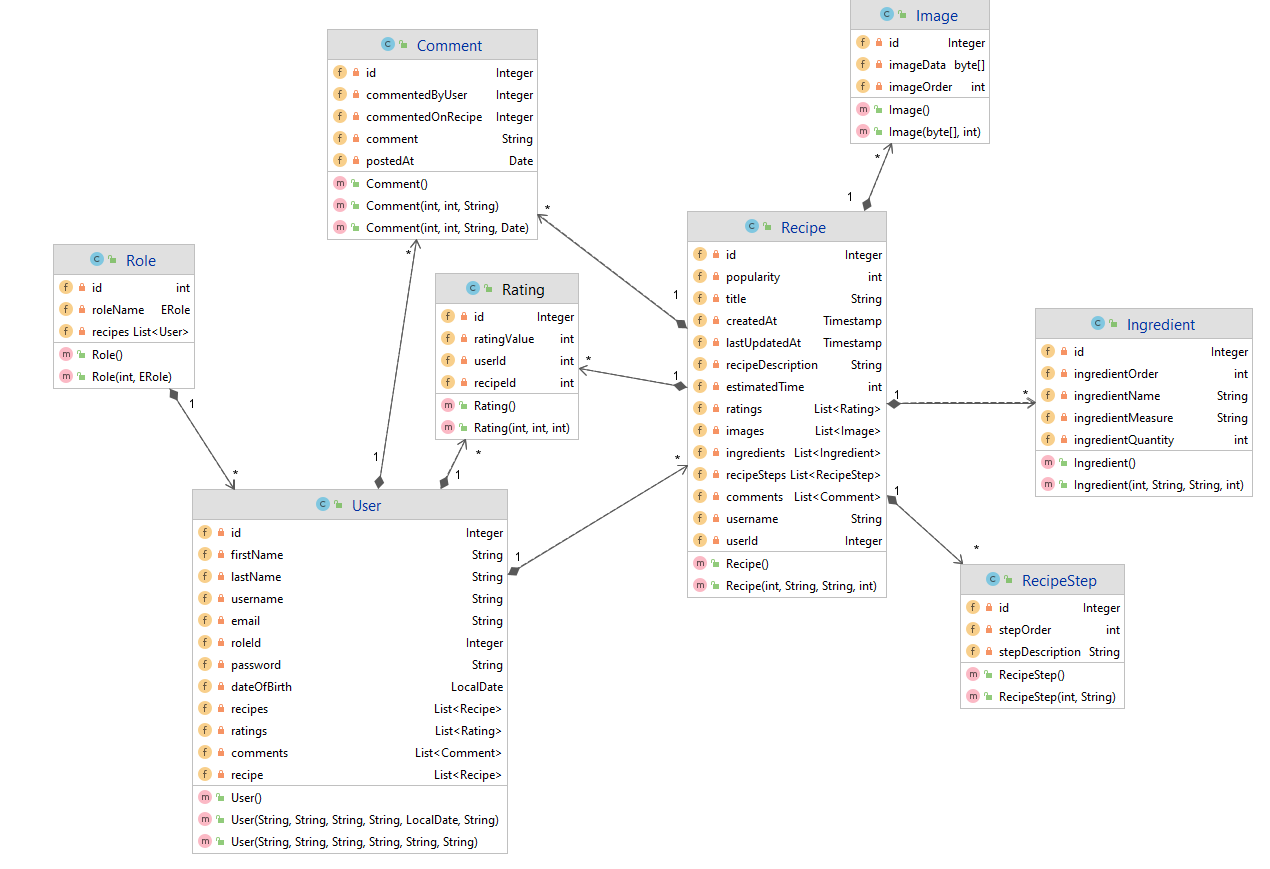
\includegraphics[scale=0.55]{slike/modelsDiagram.PNG} %veličina slike u odnosu na originalnu datoteku i pozicija slike
	\centering
	\caption{Dijagram razreda - Models}
	\label{fig:promjene}
\end{figure}

\begin{figure}[H]
	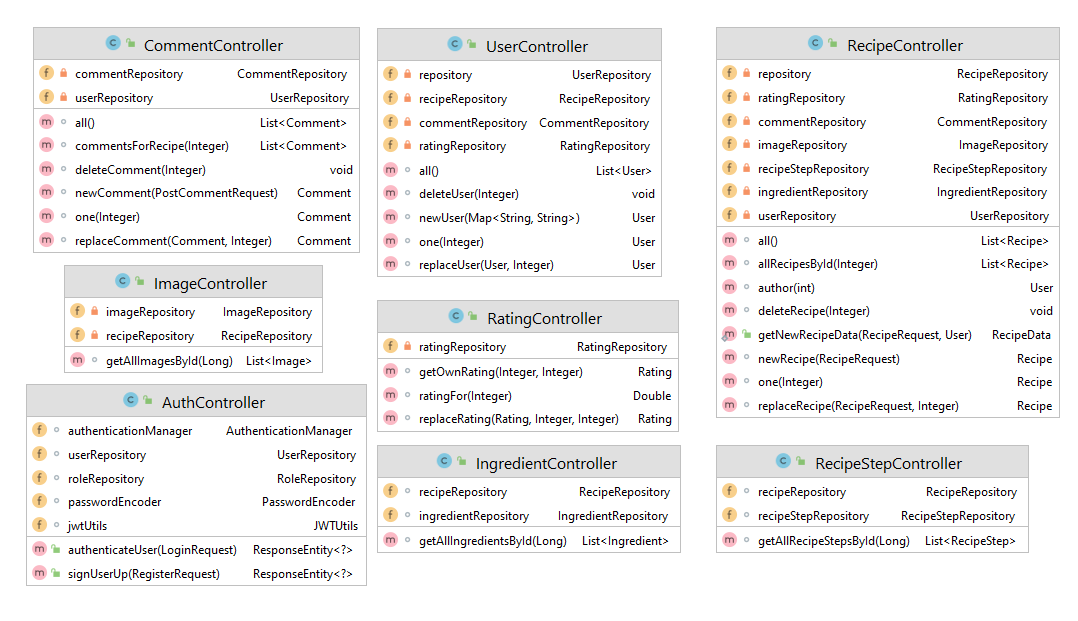
\includegraphics[scale=0.6]{slike/controllerDiagram.PNG} %veličina slike u odnosu na originalnu datoteku i pozicija slike
	\centering
	\caption{Dijagram razreda - Controllers}
	\label{fig:promjene}
\end{figure}

\begin{figure}[H]
	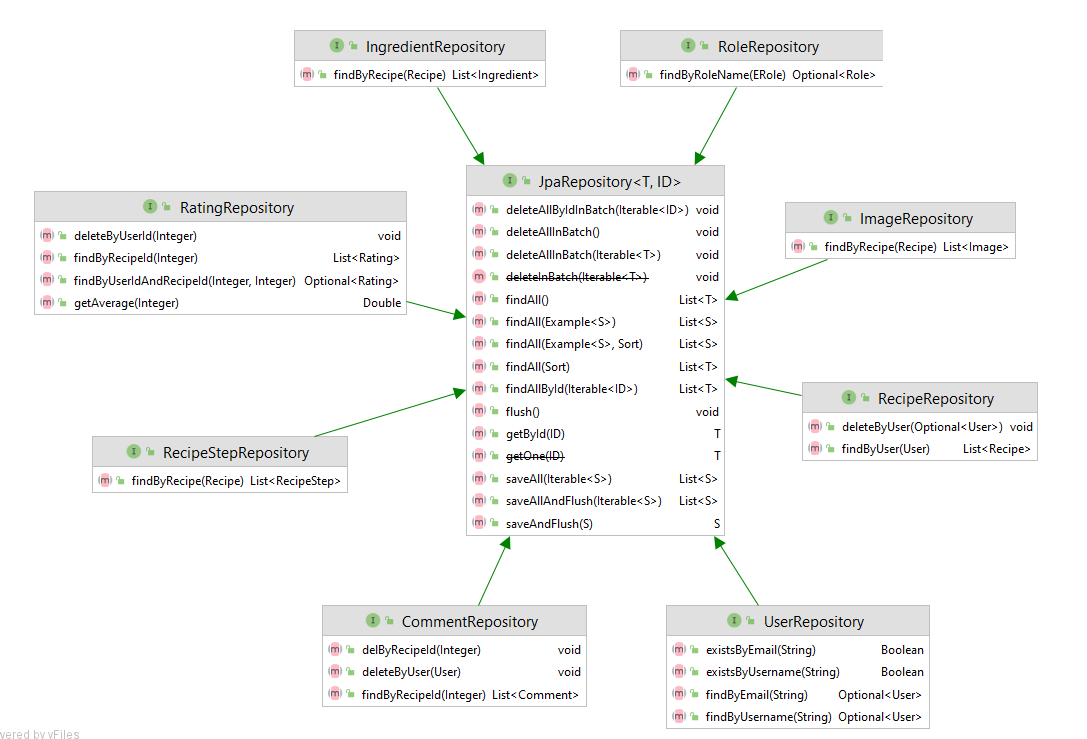
\includegraphics[scale=0.6]{slike/repositoriesDiagram.PNG} %veličina slike u odnosu na originalnu datoteku i pozicija slike
	\centering
	\caption{Dijagram razreda - Repositories}
	\label{fig:promjene}
\end{figure}


\eject

\section{Dijagram stanja}

Dijagram stanja prikazuje stanja objekta te prijelaze iz jednog stanja u drugo temeljene na događajima. Na slici 4.6 vidljiv je dijagram stanja registriranog korisnika. Korisnikove mogućnosti, osim pregleda svih recepata koji se prikazuju pri učitavanju stranice, su i pregled vlastitih recepata. Klikom na Sortiraj, korisnik može sortirati recepte po ocjeni, preporuci i popularnosti te mu je omogućen lakši pregled istih. 

Na istoj stranici, korisnik može pretražiti recepte te se tu otvaraju dvije mogućnosti, pretraživanje po sastojku te pretraživanje po imenu sve u svrhu lakšeg pretraživanja. Klijent izlistane recepte može ocijeniti, pregledati i komentirati. 
Klikom na "Moji recepti", korisniku se prikazuju svi njegovi dosadašnji recepti. Svoje recepte korisnik može obrisati, klikom na "Izbriši recept", sortirati klikom na "Sortiraj" te urediti pojedini recept.

\begin{figure}[H]
	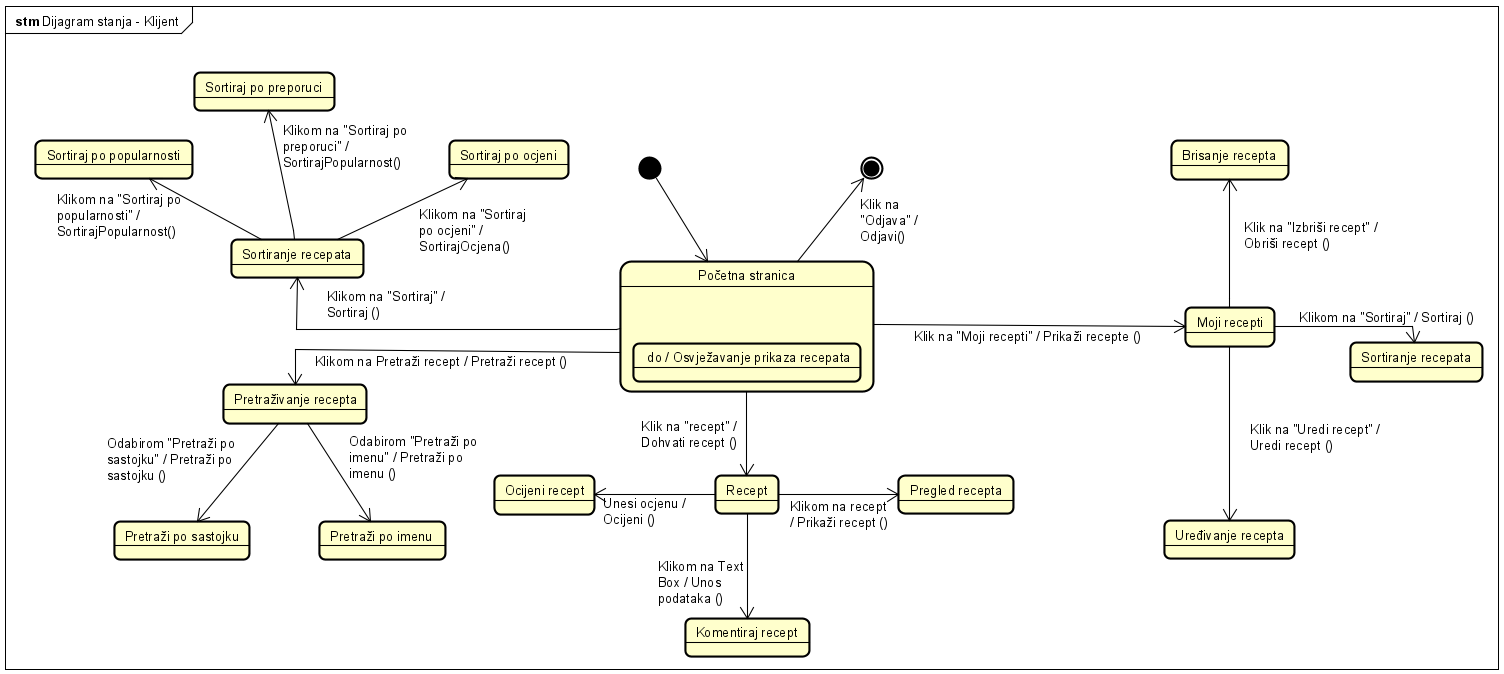
\includegraphics[scale=0.5]{slike/StateD2.PNG} %veličina slike u odnosu na originalnu datoteku i pozicija slike
	\centering
	\caption{Dijagram stanja}
	\label{fig:promjene}
\end{figure}

\eject

\section{Dijagram aktivnosti}

Dijagram aktivnosti modelira ponašanja nizom akcija. Primjenjuje se za modeliranje poslovnih procesa te upravljačkog i podatkovnog toka. Na slici 4.7 prikazan je Dijagram aktivnosti za unos novog recepta. Korisnik na početku učitava stranicu na koju nije prijavljen. Neprijavljeni korisnik i dalje ima mnoge mogućnosti ali da bi dodao svoj recept on se mora prijaviti u sustav. 

Korisnik se prijavljuje klikom na "Prijava" te se učitava stranica za prijavu. Podaci prijave se šalju Bazi podataka na validaciju te nakon njene potvrde, korisniku je omogućen daljnji pristup unosa recepta. Korisnik klikom na dodaj recept unosi podatke o receptu te pri tome mora zadovoljiti uvjete kao što su maksimalnih 5 slika koje može a i ne mora unijeti. Ujedno, potrebno je unijeti barem jedan korak pripreme te se uneseni podaci provjeravaju u Bazi podataka. Nakon zadovoljavajućeg unosa podataka recepta, šalje se poruka da je recept valjano dodan.

\begin{figure}[H]
	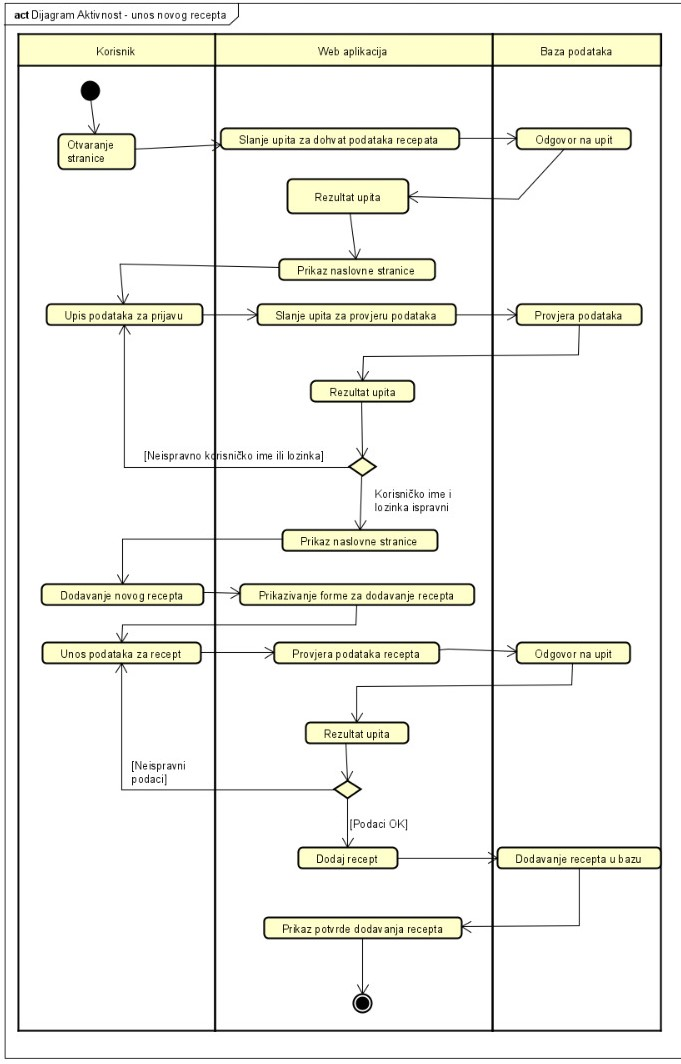
\includegraphics[scale=0.6]{slike/ActivityD.PNG} %veličina slike u odnosu na originalnu datoteku i pozicija slike
	\centering
	\caption{Dijagram aktivnosti}
	\label{fig:promjene}
\end{figure}

\eject
\section{Dijagram komponenti}

\text\noindent
Dijagram komponenti prikazan na slici 4.8 opisuje organizaciju i međusobnu ovisnost komponenti, unutrašnje strukture i odnose prema okolini.
Preko sučelja "Dohvati HTML, CSS i JS datoteke" poslužuju se datoteke za \textit{frontend} dio web aplikacije.
\textit{Frontend} dio web aplikacije se sastoji od niza TypeScript datoteka koje predstavljaju aktore koji tim datotekama mogu pristupiti.
Preko sučelja "Dohvati JSON" pristupa se REST API komponenti. REST API poslužuje podatke koje pripadaju \textit{backend} dijelu web apliakcije.
JPA Repository služi ya dohvaćanje tablica iz baze podataka koristeći SQL upite. 

\begin{figure}[H]
	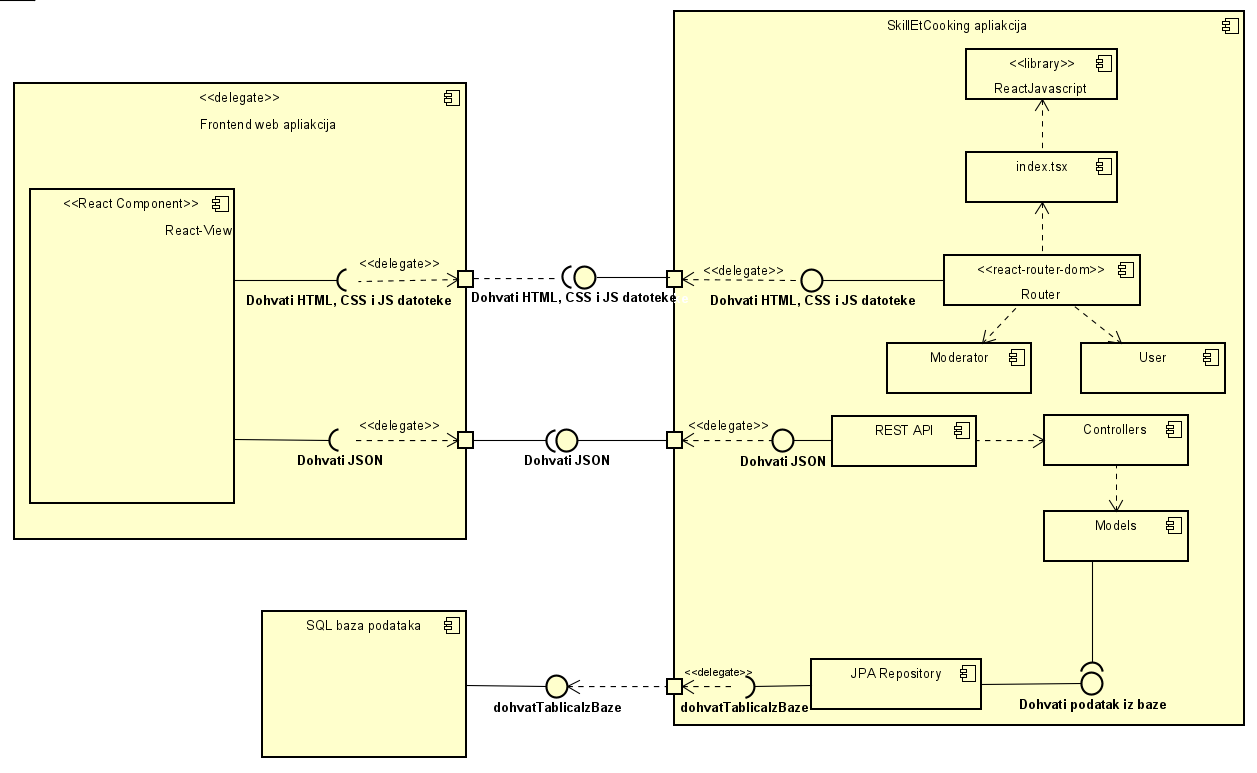
\includegraphics[scale=0.6]{slike/dijagramKomp.png} %veličina slike u odnosu na originalnu datoteku i pozicija slike
	\centering
	\caption{Dijagram komponenti}
	\label{fig:promjene}
\end{figure}
\chapter{Implementacija i korisničko sučelje}


\section{Korištene tehnologije i alati}

\text
Za potrebe komunikacije među članovima tima korištena je aplikacija \underline{WhatsApp}\footnote{https://www.whatsapp.com/}.
Za izradu UML dijagrama korišten je alat \underline{Astah Professional}\footnote{https://astah.net/products/astah-professional/},
a kao sustav za upravljanje izvornim kodom \underline{Git}\footnote{https://git-scm.com}.
Udaljeni repozitorij projekta dostupan je na web platformi \underline{GitLab}\footnote{https://about.gitlab.com}.

\text
Za razvojno okruženje odlučili smo se za \underline{Microsoft Visual Studio Code}\footnote{https://code.visualstudio.com}.
Visual Studio Code, ili kraće VSC, integrirano je razvojno okruženje (IDE) tvrtke Microsoft.
Značajke VSC-a uključuju podršku za otklanjanje pogrešaka, isticanje sintakse, inteligentno dovršavanje koda, isječke, refaktoriranje
koda i ugrađeni Git.

\text
Aplikacija je napisana koristeći radni okvir \underline{Spring Boot}\footnote{https://spring.io} i jezik
\underline{Java}\footnote{https://www.java.com/en/} za izradu \textit{backenda} te
\underline{React}\footnote{https://reactjs.org} i jezik \underline{TypeScript}\footnote{https://www.typescriptlang.org}
za izradu \textit{frontenda}.
React je biblioteka u JavaScriptu za izradu korisničkih sučelja. Održavaju ga Meta i zajednica pojedinačnih programera i tvrtki.
React se najčešće koristi kao osnova u razvoju web i mobilnih aplikacija.
React se bavi samo upravljanjem stanjem i prikazivanjem tog stanja te prilikom izrade složenijih aplikacija zahtjeva korištenje
dodatnih biblioteka za interakciju s API-jem.
Radni okvir Spring boot je sredstvo kojim se olakšava i ubrzava izrada web aplikacija.
Ima mogućnost autokonfiguracije, odlučan pristup konfiguraciji i mogućnost izrade samostalnih aplikacija.
Ove značajke rade zajedno kako bi vam pružile alat koji vam omogućuje postavljanje aplikacije koja se temelji na Springu uz minimalnu konfiguraciju i postavljanje.

\text
Baza podataka se nalazi na poslužitelju u oblaku na \underline{AWS}\footnote{https://aws.amazon.com/}


\eject


\section{Ispitivanje programskog rješenja}


\subsection{Ispitivanje komponenti}
Obavljeno je ispitavanje funkcionalnosti metoda iz klase: \textit{RecipeController.java}.
Poseban naglasak na metodi dodavanja novog recepta koja prima podatke
iz HTTP zahtjeva provjerava ih i priprema za spremanje u bazu.
Ta metoda se zove \linebreak\textit{+getNewRecipeData(RecipeRequest, User):RecipeData}
i nalazi se u razredu \textit{RecipeController.java}. Prvi ispitni slučaj je namijenjen provjeri sigurnosti
tako da se ne dopusti funkcionalnost dodavanja recepta neprijavljenim korisnicima, a u zadnjem ispitnom slučaju
je demonstrirana da ukoliko neprijavljeni korisnik pristupa domeni umjesto očekivanog odgovora: \textit{HTTP: 200 OK}
dobije se odgovor \textit{HTTP: 401 UNAUTHORIZED}. Nadalje drugi ispitni slučaj provjera je li rezultat metode
u skladu s očekivanim u slučaju kada joj se pošalju ispravni podatci. Svi ostali ispitni slučajevi ispituju rubne slučajeve i
slučajeve u kojima metoda ne smije dati nikakv rezultat nego mora baciti iznimku. Primjeri takvih slučajeva su:
slanje zahtjeva sa pet ili jednom slikom \textit{(oni predstavljaju rubne slučajeve jer je minimalan broj slika jedna, a maksimalan pet)},
slanje zahtjeva bez ijednog sastojka, slanje zahtjeva u kojima su sastojaci nepotpuni
\textit{(ne sadrže naziv, količinu ili mjernu jedinicu)}, slanje zahtjeva bez ijednog koraka pripreme...
\lstinputlisting[basicstyle=\tiny,title=Izvorni kod testova:,numbers=left]{kod/RecipeControllerTest.java}
\begin{figure}[H]
	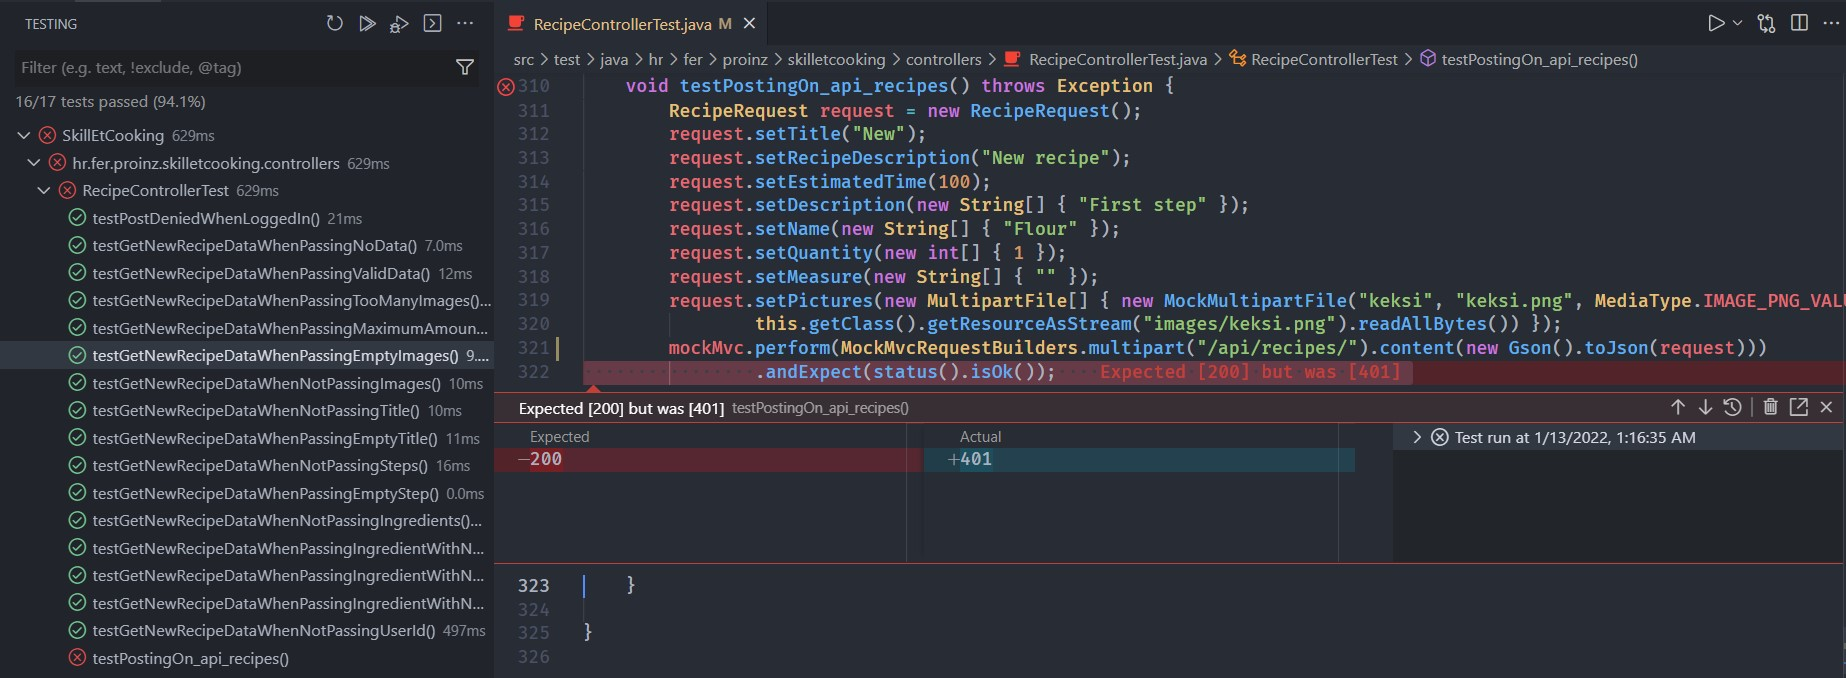
\includegraphics[scale=0.4]{slike/tests.jpg} %veličina slike u odnosu na originalnu datoteku i pozicija slike
	\centering
	\caption{Rezultati izvođenja testova u uređivaču VSCode.}
	\label{fig:promjene}
\end{figure}

\subsection{Ispitivanje sustava}
\noindent \underbar{\textbf{1. Ispitivanje prijave u sustav (UC-7)}}\break
U ovom ispitnom slučaju je provedena prijava. Scenarij započinje otvaranjem početne stranice i pod pretpostavkom da korisnik
nije prijavljen u sustav biti će vidljiva hiperveza koja vodi na stranicu za prijavu. Nakon toga unošenjem korisničkog imena
i lozinke te klikom na gumb za prijavu korisnik bi trebao biti preusmjeren na početnu stranicu ali ovaj put uz dodatne mogućnosti
što se provjerava postojanjem hiperveze koja vodi na vlastite recepte.
\begin{figure}[H]
	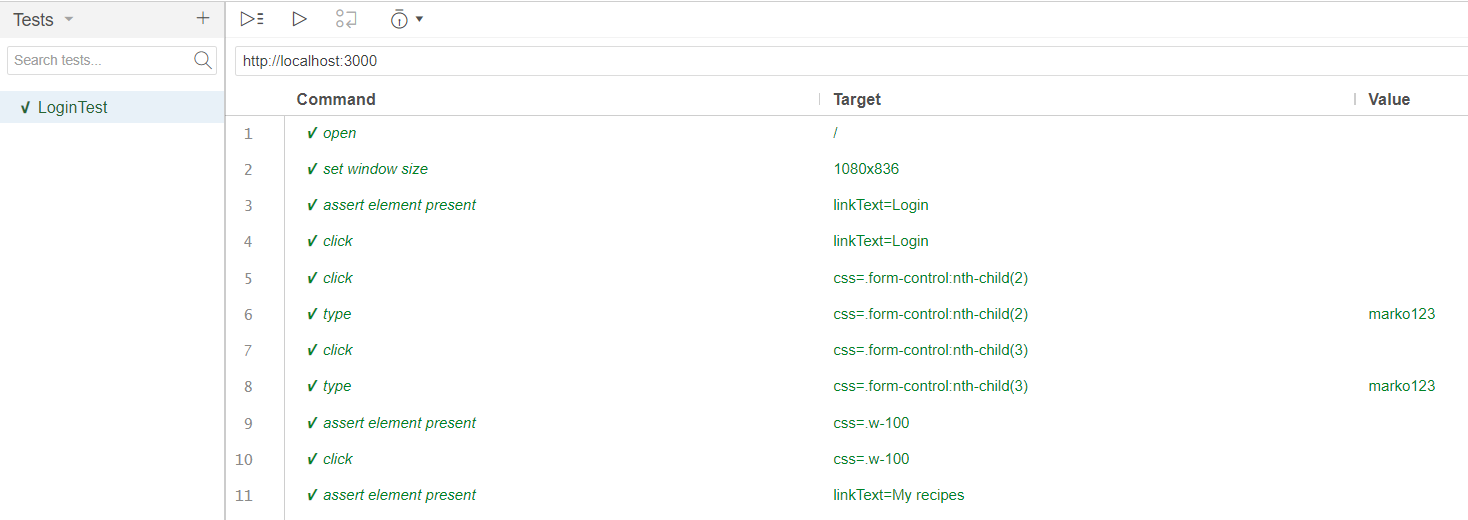
\includegraphics[scale=0.6]{slike/login.png} %veličina slike u odnosu na originalnu datoteku i pozicija slike
	\centering
	\caption{Ispitivanje prijave u sustav.}
	\label{fig:promjene}
\end{figure}

\noindent \underbar{\textbf{2. Ispitivanje pretraživanja recepta po sastojcima (UC-5)}}\break
U ovom ispitnom slučaju je provedeno pretraživanje recepata po sastojcima. Scenarij započinje
otvaranjem početne stranice na kojoj se nalazi HTML element za unos sastojaka. Pod pretpostavkom
da u bazi postoji recept sa sastojcima: peršin, češnjak, špageti i vrhnje (za-kuhanje),
nakon odabira upravo tih sastojaka na početnoj stranici bi trebao biti vidljiv taj recept što se
provjerava njegovom prisutnošću.
\begin{figure}[H]
	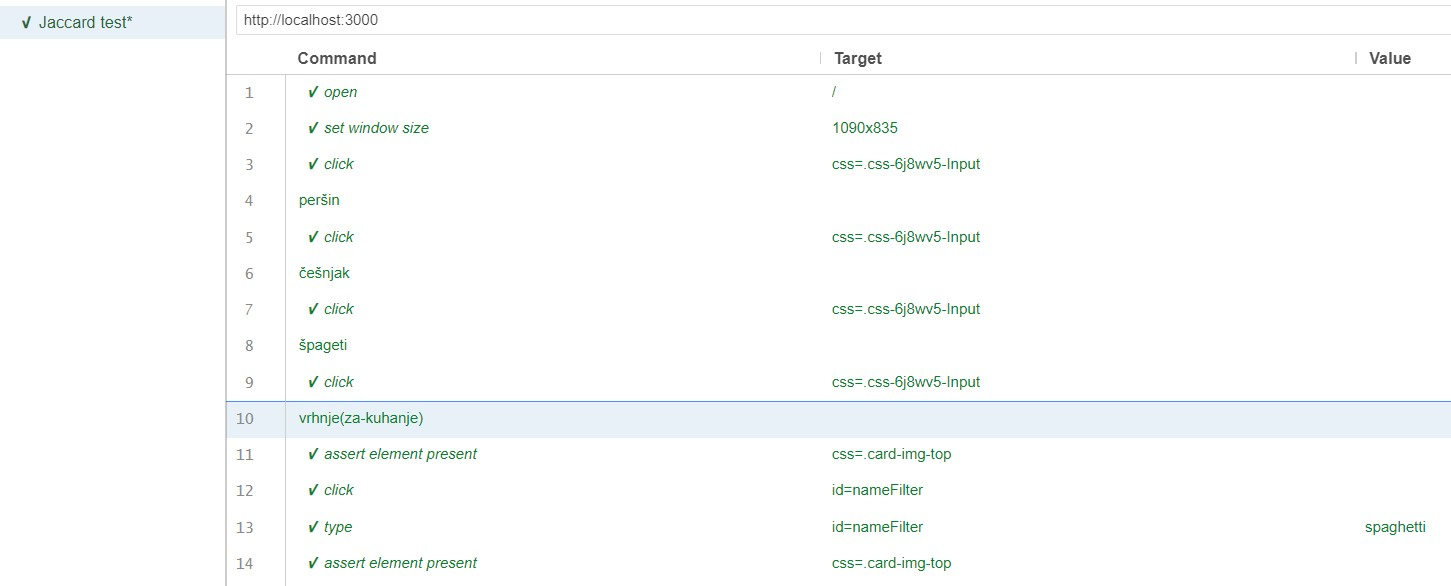
\includegraphics[scale=0.6]{slike/jaccard.jpg} %veličina slike u odnosu na originalnu datoteku i pozicija slike
	\centering
	\caption{Ispitivanje pretraživanja recepata po sastojcima.}
	\label{fig:promjene}
\end{figure}

\newpage

\noindent \underbar{\textbf{3. Ispitivanje registracije u sustav (UC-6)}}\break
U ovom ispitnom slučaju je provedena registracija korisnika u sustav. Scenarij započinje otvaranjem početne
stranice gdje su prikazani svi recepti. Nakon toga korisnik odabire hipervezu registracija koja
ga vodi na formu za registraciju. Korisnik popunjava podatke te ako su zadovoljeni svi uvjeti
korisnik će biti uspješno registriran te će ga se potom preusmjeriti na početnu stranicu,
ali će ovaj put biti prijavljen u sustav. Nakon toga će biti vidljiva hiperveza My recipes
koja se pojavljuje samo prijavljenim korisnicima.
\begin{figure}[H]
	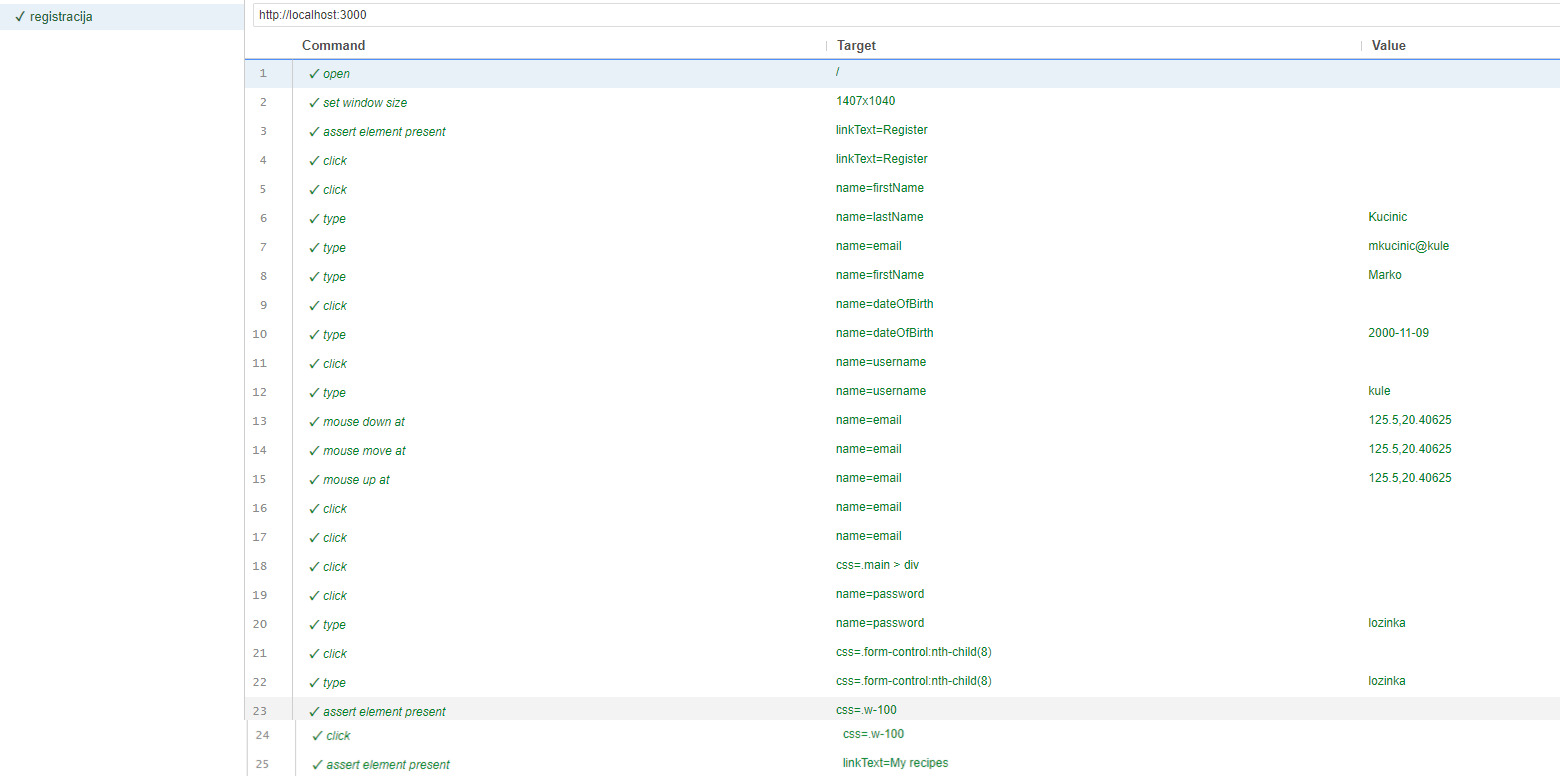
\includegraphics[scale=0.2]{slike/registracija1.png} %veličina slike u odnosu na originalnu datoteku i pozicija slike
	\centering
	\caption{Ispitivanje registracije u sustav.}
	\label{fig:promjene}
\end{figure}

\noindent \underbar{\textbf{4. Ispitivanje dodavanja komentara moderatora (UC-14)}}\break
U ovom ispitnom slučaju je provedeno dodavanje komentara moderatora. Moderator se poput ostalih
korisnika mora prijaviti u sustav. Nakon prijave moderator odabire opciju prikaza određenog
recepta. U polju za komentare upisuje komentar po želji i pritiskom na hipervezu objavi
komentar dodaje komentar u bazu. Pritiskom na tipku osvježi komentar će se prikazati uz
ostale komentare toga recepta. Također, komentar će biti dodatno naglašen oznakom za moderatore (kruna).
\begin{figure}[H]
	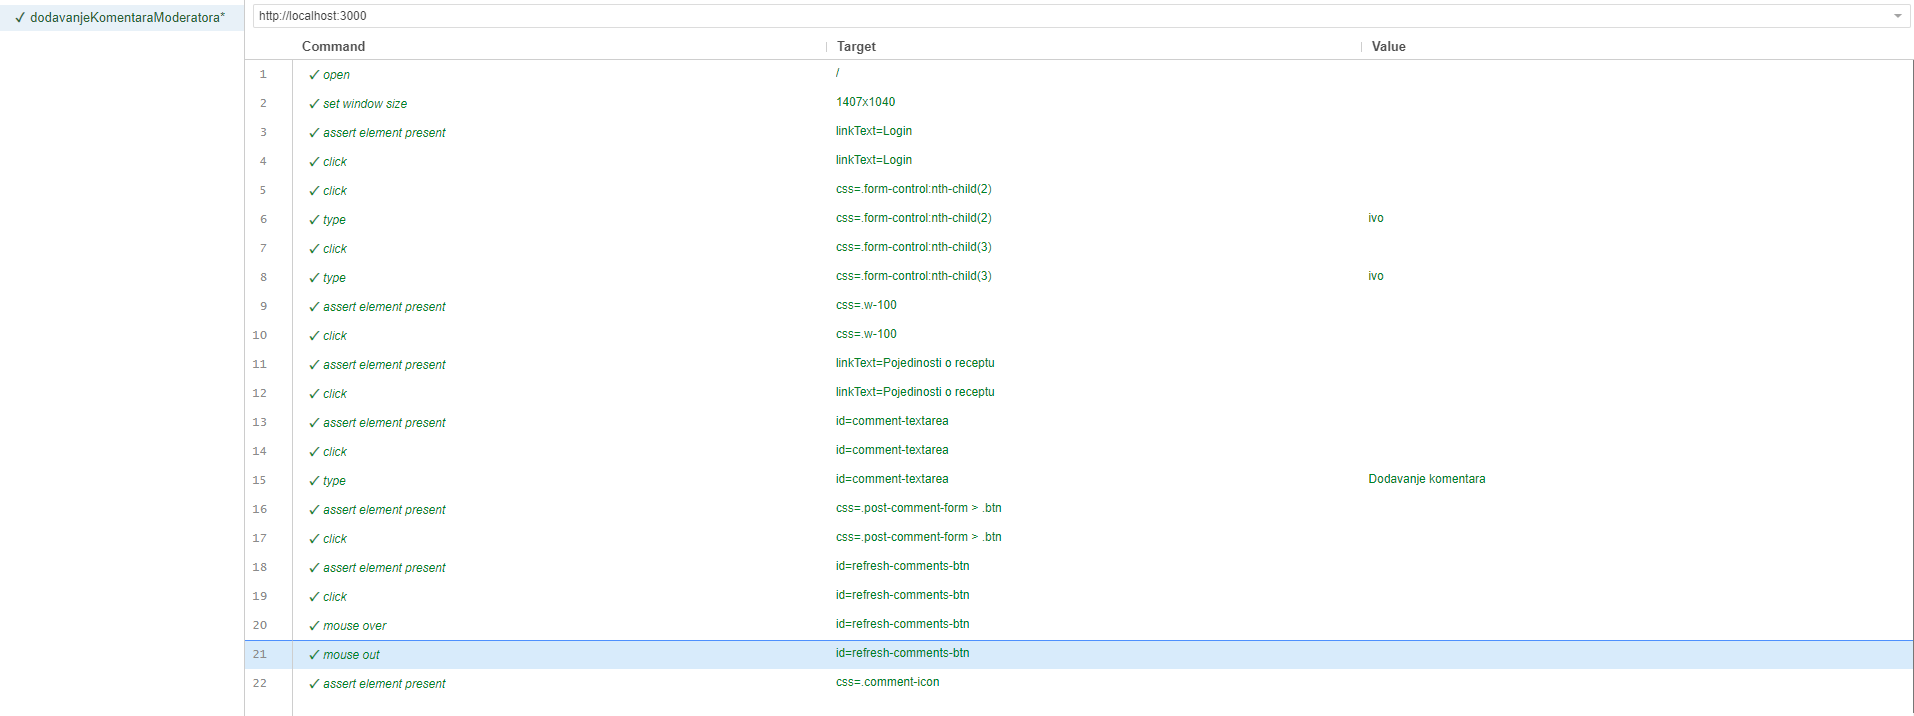
\includegraphics[scale=0.4]{slike/dodavanjeKomentaraModeratora.png.jpg} %veličina slike u odnosu na originalnu datoteku i pozicija slike
	\centering
	\caption{Ispitivanje dodavanja komentara moderatora.}
	\label{fig:promjene}
\end{figure}

\eject


\section{Dijagram razmještaja}

Dijagrami razmještaja opisuju topologiju sklopovlja i programsku potporu koja se koristi u implementaciji sustava u njegovom radnom okruženju. Upogonjenje smo izvršili na AWS-u pa imamo dijagram s 3 uređaja. Servis web poslužitelja pokrenut je na Amazon EC2 instanci koji s bazom pokrenutoj preko Amazon RDS-a komunicira preko TCP protokola na vratima 5432. Klijenti koriste web preglednik na vlastitim računalima kako pi pristupili web aplikaciji. Sustav je baziran na arhitekturi "klijent -poslužitelj", a komunikacija između računala korisnika i poslužitelja odvija se preko HTTP veze.
\begin{figure}[H]
	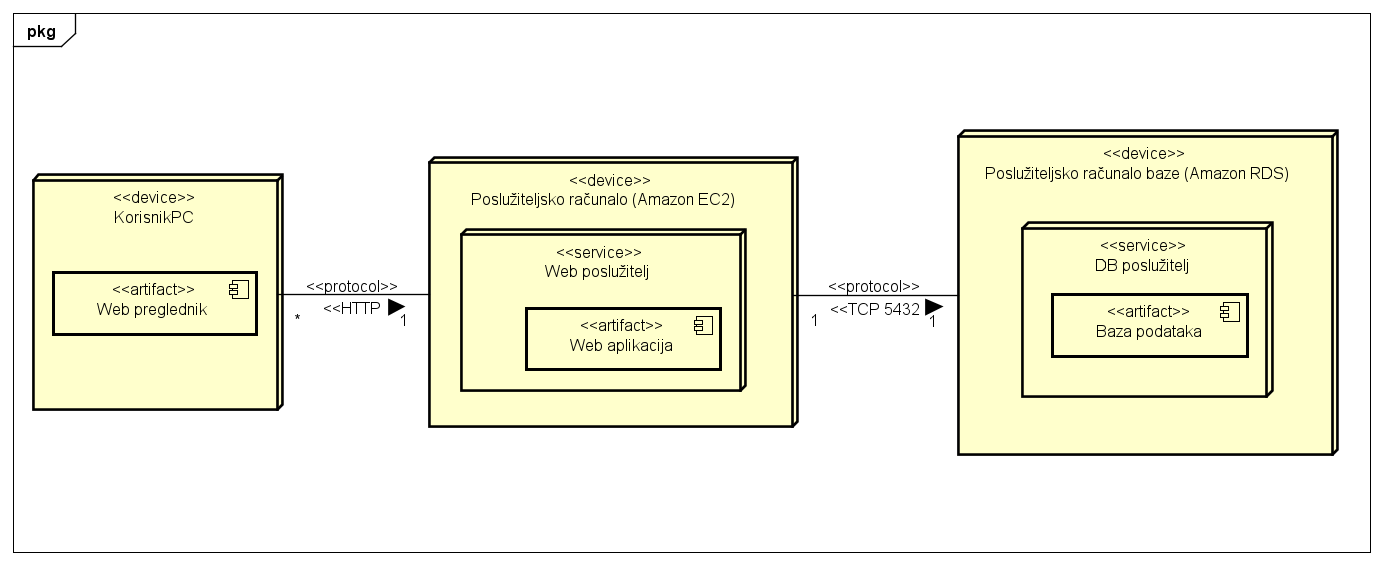
\includegraphics[scale=0.45]{slike/DijagramRazmjestaja.PNG} %veličina slike u odnosu na originalnu datoteku i pozicija slike
	\centering
	\caption{Dijagram razmještaja}
	\label{fig:promjene}
\end{figure}
\eject

\section{Upute za puštanje u pogon}

\lstset{
	backgroundcolor=\color{white},   % choose the background color; you must add     \usepackage{color} or \usepackage{xcolor}; should come as last argument
	basicstyle=\footnotesize,        % the size of the fonts that are used for the code
	breakatwhitespace=false,         % sets if automatic breaks should only happen at whitespace
	breaklines=true,                 % sets automatic line breaking
	captionpos=t,                    % sets the caption-position to top
	deletekeywords={...},            % if you want to delete keywords from the given language
	escapeinside={\%*}{*)},          % if you want to add LaTeX within your code
	extendedchars=true,              % lets you use non-ASCII characters; for 8-bits encodings only, does not work with UTF-8
	frame=single,                      % adds a frame around the code
	keepspaces=true,                 % keeps spaces in text, useful for keeping indentation of code (possibly needs columns=flexible)
	keywordstyle=\color{blue},       % keyword style
	morekeywords={*,...},            % if you want to add more keywords to the set
	rulecolor=\color{black},         % if not set, the frame-color may be changed on line-breaks within not-black text (e.g. comments (green here))
	showspaces=false,                % show spaces everywhere adding particular underscores; it overrides 'showstringspaces'
	showstringspaces=false,          % underline spaces within strings only
	showtabs=false,                  % show tabs within strings adding particular underscores
	tabsize=2,                     % sets default tabsize to 2 spaces
	title=\lstname                   % show the filename of files included with \lstinputlisting; also try caption instead of title
}
\hfill \break
\textbf{Instalacija potrebnih programa}\\
Prije lokalnog pokretanja potrebno je instalirati sljedeće programske alate:
\begin{itemize}
	\item Node + NPM
	\item Java 11
	\item Maven
	\item PostgreSQL 12 + PgAdmin
	\item git
\end{itemize}

Za kloniranje repozitorija i koda koristimo sljedeću naredbu te se autenticiramo našim GitLab podacima:
\begin{lstlisting}[]
git clone https://gitlab.com/progimeri/proinz-projekt.git
\end{lstlisting}
\hfill \break
\hfill \break
\textbf{Konfiguracija baze podataka}\\

Prije pokretanja same web aplikacije moramo konfigurirati lokalnu bazu podataka. Konfiguraciju poslužitelja baze možemo napraviti proizvoljno te poslije specificirati u kodu, ali preporuča se korištenje zadanih podataka:
\begin{figure}[H]
	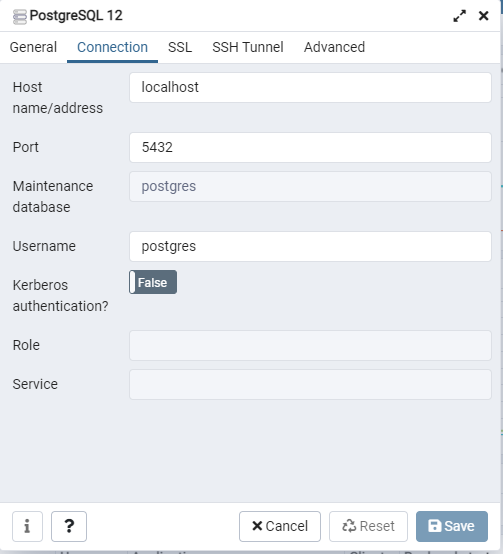
\includegraphics[scale=1]{slike/server_properties.PNG} %veličina slike u odnosu na originalnu datoteku i pozicija slike
	\centering
	\caption{Postavke poslužitelja baze}
	\label{fig:promjene}
\end{figure}
Nakon stvaranja poslužitelja baze možemo stvoriti bazu bilo kojeg imena, ali preporuka je koristiti ime 'skilletcooking' s vlasnikom 'postgres':
\begin{figure}[H]
	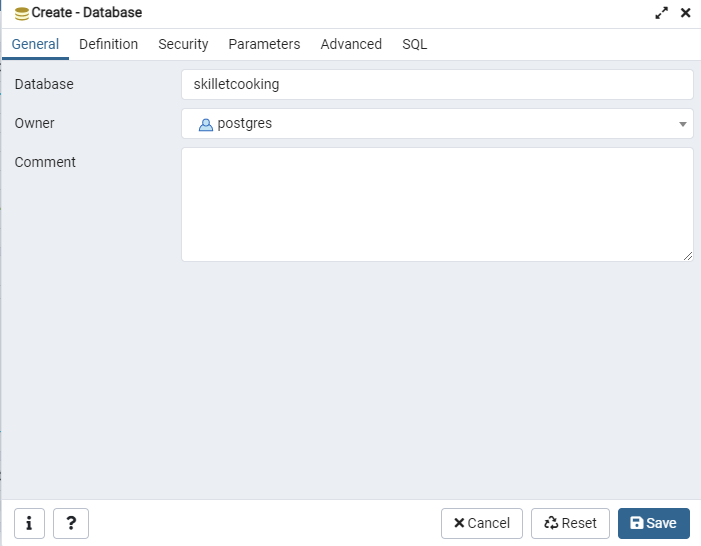
\includegraphics[scale=0.8]{slike/database_properties.PNG} %veličina slike u odnosu na originalnu datoteku i pozicija slike
	\centering
	\caption{Postavke baze podataka}
	\label{fig:promjene}
\end{figure}
\hfill \break
\textbf{Konfiguracija stražnjeg dijela}\\
Samu shemu baze popuniti će Flyway migracija prilikom prvog pokretanja back-end poslužitelja. Kako bi poslužitelj spojili na lokalnu bazu podataka trebamo definirati da je aktivni profil dev u application.properties datoteci:
\begin{lstlisting}
spring.profiles.active=dev
\end{lstlisting}

Samim time ako se zbog nekog razloga želimo spojiti na bazu podataka koja je pokrenuta na AWS-u to možemo jednostavno tako da zamijenimo aktivni profil sa prod:
\begin{lstlisting}
spring.profiles.active=prod
\end{lstlisting}

Prijašnje postavke koje smo definirali pri izradi baze podataka sada moramo specificirati u application-dev.properties datoteci u izvornom kodu back-enda i izmijeniti sljedeće linije.
\lstset{}
\begin{lstlisting}[]
spring.datasource.url=jdbc:postgresql://{host_name}/{database_name}
spring.datasource.username={database_user_name}
spring.datasource.password={lozinka}

spring.flyway.url=jdbc:postgresql://{host_name}/{database_name}
spring.flyway.user={database_user_name}
spring.flyway.password={lozinka}
\end{lstlisting}

Za predložene podatke i korisnika postgres kojemu je lozinka 'bazepodataka' to bi izgledalo ovako:
\begin{lstlisting}[]
spring.datasource.url=jdbc:postgresql://localhost:5432/skilletcooking
spring.datasource.username=postgres
spring.datasource.password=bazepodataka

spring.flyway.url=jdbc:postgresql://localhost:5432/skilletcooking
spring.flyway.user=postgres
spring.flyway.password=bazepodataka
\end{lstlisting}
Kada je cijela konfiguracija namještena napokon možemo pokrenuti back-end koji će pokrenuti generiranje sheme u bazi. To možemo tako da se u konzoli pozicioniramo u mapu izvorniKod/back-end i pokrenemo naredbu \lstinline|mvn spring-boot:run| koja će pokrenuti Java Spring poslužitelj na vratima 8080. Back-end se također može pokrenuti korištenjem modernih naprednih IDE-jeva poput IntelliJ-a.\\
Kada je servis uspješno pokrenut i nakon popunjenja sheme još jedan preduvjet prije pokretanja cjelokupne aplikacije je definicija "uloga" koje korisnici mogu imati, a to su \textbf{USER} i \textbf{MODERATOR}. Te uloge možemo jednostavno dodati korištenjem alata za upite u PgAdminu i pokretanju sljedećih upita:
\begin{lstlisting}[language=sql]
INSERT INTO roles(role_name) VALUES ('USER');
INSERT INTO roles(role_name) VALUES ('MODERATOR');
\end{lstlisting}
\textbf{Pokretanje prednjeg dijela}\\
Sada je cijeli back-end spreman i možemo pokrenuti front-end. Pokrenimo novu konzolu i pozicioniramo se u mapu izvorniKod/front-end. Pokrećemo naredbu \lstinline|npm install| koja će instalirati sve potrebne pakete s npm-a te nakon toga možemo izvršiti naredbu \lstinline|npm start| koja će pokrenuti poslužitelj za prednju stranu na vratima 3000 i njemu možemo pristupiti na adresi localhost:3000.

\hfill \break
\textbf{Javni poslužitelj}\\
Aplikacija je pokrenuta na javnom poslužitelju preko AWS-a i dostupna je na stranici: http://34.244.45.75/ .
\eject
\chapter{Zaključak i budući rad}
		
	\text
	Zadatak naše grupe bio je razvoj web aplikacije za pregled recepata uz mogućnost sortiranja, 
	filtriranja, dodavanja vlastitih recepata, komentiranja i ocijenjivanja recepata. Za ovaj projekt dobili smo vrijeme od 17 tjedana.
	Za to vrijeme naš je tim uspješno završio zadatak i razvio zadanu aplikaciju. Tijek odvijanja projekta može se podijeliti u 2 faze.

	\text
	Prva faza je faza okupljanja tima i rad na zahtjevima projekta. Dokumentiranje zahtjeva je olakšalo kasniju preraspodjelu poslova
	kao i lakše osmišljavanje izgleda i funkcionalnosti web aplikacije. Kasniji problemi u drugoj fazi prilikom izrade web aplikacije 
	su se lakše rješavali uz pomoć već postojećih dijagrama čime smo smanjili gubitak vremena.

	\text
	Druga faza uključivala je izradu i isptivanje web aplikacije uz dokumentiranje projekta. Naglasak je više bio na samostalnome radu
	za razliku od prve faze zbog čega je ponekad dolazilo do problema. Neiskustvo u radu u timu kao i u radu na projektu je predstavljao
	najveći izazov, ali su svi članovi bili tu jedni za druge te nije bilo pretjeranih problema.

	\text
	Komunikacija u timu je bila jako dobra. Svi članovi tima bili su pozitivni i nije dolazilo do neželjenih sukoba.

	\text
	Sudjelovanje u ovakvome projektu bilo je od iznimne koristi svim članovima tima. Budući da je svatko radio u svim fazama i na svim 
	dijelovima web aplikacije, puno smo toga imali prilike naučiti. Raditi na ovome projektu bilo je dobro iskustvo i za buduće
	timske radove.

	\eject
\chapter*{Popis literature}
		\addcontentsline{toc}{chapter}{Popis literature}
	 	
 		\textbf{\textit{Kontinuirano osvježavanje}}
	
		\textit{Popisati sve reference i literaturu koja je pomogla pri ostvarivanju projekta.}
		
		
		\begin{enumerate}
			
			
			\item  Programsko inženjerstvo, FER ZEMRIS, \url{http://www.fer.hr/predmet/proinz}
			
			\item  I. Sommerville, "Software engineering", 8th ed, Addison Wesley, 2007.
			
			\item  T.C.Lethbridge, R.Langaniere, "Object-Oriented Software Engineering", 2nd ed. McGraw-Hill, 2005.
			
			\item  I. Marsic, Software engineering book``, Department of Electrical and Computer Engineering, Rutgers University, \url{http://www.ece.rutgers.edu/~marsic/books/SE}
			
			\item  The Unified Modeling Language, \url{https://www.uml-diagrams.org/}
			
			\item  Astah Community, \url{http://astah.net/editions/uml-new}
		\end{enumerate}
		
		 


\begingroup
\renewcommand*\listfigurename{Indeks slika i dijagrama}
%\renewcommand*\listtablename{Indeks tablica}
%\let\clearpage\relax
\listoffigures
%\vspace{10mm}
%\listoftables
\endgroup
\addcontentsline{toc}{chapter}{Indeks slika i dijagrama}



\eject

\chapter*{Dodatak: Prikaz aktivnosti grupe}
		\addcontentsline{toc}{chapter}{Dodatak: Prikaz aktivnosti grupe}
		
		\section*{Dnevnik sastajanja}

		\begin{packed_enum}
			\item  sastanak
			
			\item[] \begin{packed_item}
				\item Datum: 4. listopada 2021.
				\item Prisustvovali: K.Frankola, B.Colarić, D.Dugonjevac, T.Serezlija, M.Tunjić
				\item Teme sastanka:
				\begin{packed_item}
					\item  Međusobno upoznavanje i predstavljanje
					\item  Rasprava o projektu i zajedničkim aktivnostima (u grubo)
					\item  Prijava na stranicu raspodjele grupa
				\end{packed_item}
			\end{packed_item}
			
			\item  sastanak
			\item[] \begin{packed_item}
				\item Datum: 11. listopada 2021.
				\item Prisustvovali: K.Frankola, J.Brkić, B.Colarić, D.Dugonjevac, P.Gavran, T.Serezlija, M.Tunjić
				\item Teme sastanka:
				\begin{packed_item}
					\item  Upoznavanje novih članova
					\item  Ponovna rasprava o odabranim tehnologijama
					\item  Podjela aktivnosti po članovima
				\end{packed_item}
			\end{packed_item}
		
					\item  sastanak
		\item[] \begin{packed_item}
			\item Datum: 27. listopada 2021.
			\item Prisustvovali: K.Frankola, J.Brkić, B.Colarić, D.Dugonjevac, P.Gavran, T.Serezlija, M.Tunjić
			\item Teme sastanka:
			\begin{packed_item}
				\item  Daljnja podjela aktivnosti (dokumentacija i programiranje)
				\item  Razmatranje arhitekture i ponašanja sustava
			\end{packed_item}
		\end{packed_item}
	
						\item  sastanak
	\item[] \begin{packed_item}
		\item Datum: 6. studenoga 2021.
		\item Prisustvovali: K.Frankola, J.Brkić, B.Colarić, D.Dugonjevac, P.Gavran, T.Serezlija, M.Tunjić
		\item Teme sastanka:
		\begin{packed_item}
			\item  Osnovni dijagram baze
			\item  Osnovni dijagram ponašanja sustava
			\item  Aktivnosti koje je potrebno napraviti do predaje
		\end{packed_item}
	\end{packed_item}

						\item  sastanak
\item[] \begin{packed_item}
	\item Datum: 9. prosinca 2021.
	\item Prisustvovali: K.Frankola, J.Brkić, B.Colarić, D.Dugonjevac, P.Gavran, T.Serezlija, M.Tunjić
	\item Teme sastanka:
	\begin{packed_item}
		\item  Podjela aktivnosti za alfa verziju
	\end{packed_item}
\end{packed_item}

						\item  sastanak
\item[] \begin{packed_item}
	\item Datum: 10. siječnja 2022.
	\item Prisustvovali: K.Frankola, J.Brkić, B.Colarić, D.Dugonjevac, P.Gavran, T.Serezlija, M.Tunjić
	\item Teme sastanka:
	\begin{packed_item}
		\item  Finalni dogovori oko podjele zadataka
		\item  Završavanje implementacije i nedostatci
	\end{packed_item}
\end{packed_item}
			
			%
			
		\end{packed_enum}
		
		\eject
		\section*{Tablica aktivnosti}
		
			\textbf{\textit{Kontinuirano osvježavanje}}\\
			
			 \textit{Napomena: Doprinose u aktivnostima treba navesti u satima po članovima grupe po aktivnosti.}

			\begin{longtblr}[
					label=none,
				]{
					vlines,hlines,
					width = \textwidth,
					colspec={X[7, l]X[1, c]X[1, c]X[1, c]X[1, c]X[1, c]X[1, c]X[1, c]}, 
					vline{1} = {1}{text=\clap{}},
					hline{1} = {1}{text=\clap{}},
					rowhead = 1,
				} 
				\multicolumn{1}{c|}{} & \multicolumn{1}{c|}{\rotatebox{90}{\textbf{Karlo Frankola }}} & \multicolumn{1}{c|}{\rotatebox{90}{\textbf{Jan Brkić }}} &	\multicolumn{1}{c|}{\rotatebox{90}{\textbf{Borna Colarić }}} & \multicolumn{1}{c|}{\rotatebox{90}{\textbf{Dario Dugonjevac }}} &	\multicolumn{1}{c|}{\rotatebox{90}{\textbf{Petar Gavran }}} & \multicolumn{1}{c|}{\rotatebox{90}{\textbf{Toni Serezlija }}} &	\multicolumn{1}{c|}{\rotatebox{90}{\textbf{Marko Tunjić }}} \\  
				Upravljanje projektom 		& 8 &  &  &  &  &  & \\ 
				Opis projektnog zadatka 	&  &  & 1 & 2 &  &  & 2 \\ 
				
				Funkcionalni zahtjevi       &  &  & 3 &  &  &  & 2  \\ 
				Opis pojedinih obrazaca 	&  &  &  &  &  & 3 &  \\ 
				Dijagram obrazaca 			&  &  &  &  &  &  & 1  \\ 
				Sekvencijski dijagrami 		&  &  &  & 2 &  &  &  \\ 
				Opis ostalih zahtjeva 		&  &  &  &  &  & 1 &  \\ 

				Arhitektura i dizajn sustava	 &  &  &  &  &  & 2 &  \\ 
				Baza podataka				&  &  &  &  &  & 2 &   \\ 
				Dijagram razreda 			& 1 & 1.5  &  &  &  &  &   \\ 
				Dijagram stanja				&  & 1 &  &  &  &  &  \\ 
				Dijagram aktivnosti 		&  & 1 &  &  &  &  &  \\ 
				Dijagram komponenti			&  &  &  & 1 &  &  &  \\ 
				Korištene tehnologije i alati 		&  & 1 &  &  &  &  &  \\ 
				Ispitivanje programskog rješenja 	&  &  &  &  &  & 4 &  \\ 
				Dijagram razmještaja			& 1  &  &  &  &  &  &  \\ 
				Upute za puštanje u pogon 		& 1  &  &  &  &  &  &  \\  
				Dnevnik sastajanja 			& 1 &  &  &  &  &  &  \\ 
				Zaključak i budući rad 		&  &  &  & 1 &  &  &  \\  
				Popis literature 			&  &  &  &  &  &  &  \\ \hline 
				\textit{Izrada početne stranice}  & 4 & 1 &  &  &  &  &  \\  
				\textit{Izrada baze podataka} & 2 &  & 1 & 1 &  & 1 & 1\\  
				\textit{Spajanje s bazom podataka} 	& 2 &  &  &  &  &  &  \\ 
				\textit{Back End}	& 12 &  & 7 & 7 &  & 7  & 8  \\  
				\textit{Front End}  & 8 & 7 & 3 & 7 &  & 8 & 7 \\
				\textit{Puštanje u pogon} & 7 & & & & & & \\ 
			\end{longtblr}
					
					
		\eject
		\section*{Dijagrami pregleda promjena}
		
		\begin{figure}[H]
			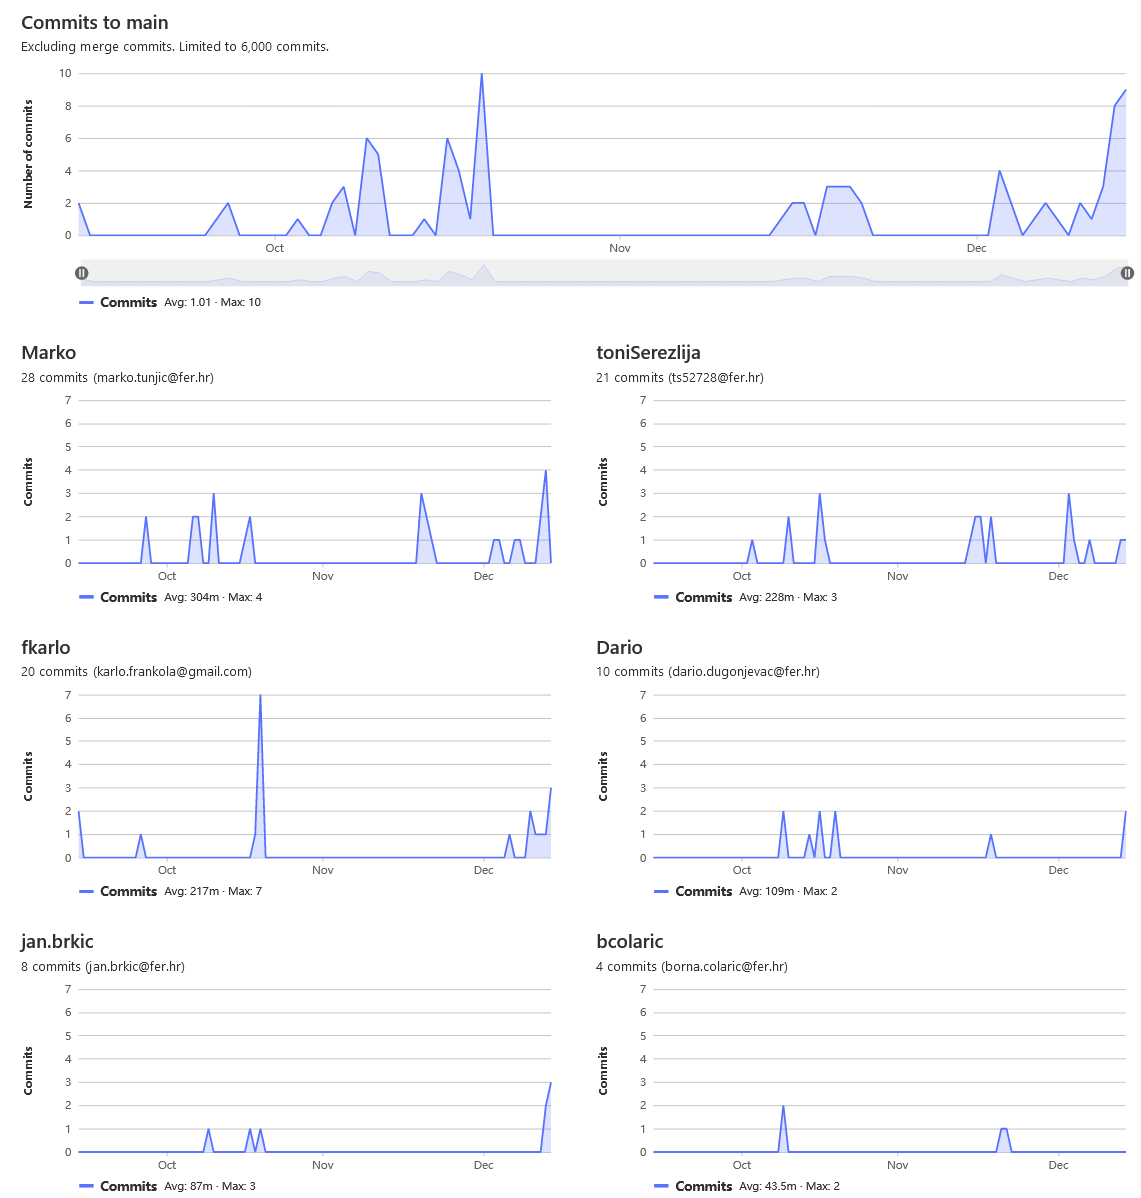
\includegraphics[scale=0.4]{slike/mainAktivnost.png} %veličina slike u odnosu na originalnu datoteku i pozicija slike
			\centering
			\caption{Aktivnost}
			\label{fig:promjene}
		\end{figure}

		
	


\end{document} %naredbe i tekst nakon ove naredbe ne ulaze u izgrađen dokument


